\chapter{Aplicaciones de la Derivada}

La derivada no es únicamente un objeto teórico: es el instrumento
central para analizar el comportamiento de funciones y resolver
problemas cuantitativos en física, ingeniería, economía y geometría.
Este capítulo desarrolla las aplicaciones más importantes, organizadas
en un orden pedagógico natural: primero el análisis del comportamiento
local (extremos, monotonía, concavidad), luego las aplicaciones al
trazado sistemático de curvas y a la optimización, y finalmente las
herramientas analíticas transversales (Teorema del Valor Medio, regla
de L'Hôpital) y numéricas (Newton-Raphson, bisección).

\begin{rem}
El hilo conductor de este capítulo es el siguiente principio: la
derivada mide la \textbf{tasa de variación instantánea}. Según el
contexto, esta idea adquiere formas distintas como lo son la velocidad, pendiente de la recta tangente, el
crecimiento marginal y la tasa de llenado pero el aparato matemático
es siempre el mismo. Reconocer esta unidad subyacente facilita la
transferencia de las técnicas entre contextos aparentemente dispares.
\end{rem}

%%==========================================================
\section{Razones de Cambio Relacionadas}
%%==========================================================

Si una cantidad $y$ depende del tiempo $t$, su derivada $\frac{dy}{dt}$
es su \textbf{razón de cambio respecto al tiempo}. Cuando dos o más
cantidades están ligadas por una ecuación geométrica o física, sus
derivadas temporales también están ligadas: son las llamadas
\textbf{razones de cambio relacionadas}. La clave es que la ecuación
que relaciona las cantidades vale para \emph{todo instante} $t$, por
lo que puede derivarse implícitamente respecto a $t$.

\begin{pasos} Las razones de cambio relacionadas pueden resolverse siguiendo el siguiente protocolo:
\begin{enumerate}
    \item \textbf{Diagrama y variables.} Dibujar un esquema de la
    situación y asignar variables a las cantidades que cambian con $t$.
    \item \textbf{Identificar razones.} Listar las derivadas temporales
    conocidas y la que se desea encontrar.
    \item \textbf{Ecuación fundamental.} Escribir una ecuación que
    relacione las variables y que sea válida para todo $t$.
    \item \textbf{Derivación implícita.} Derivar ambos lados respecto
    a $t$ aplicando la regla de la cadena.
    \item \textbf{Sustitución y despeje.} Solo \emph{después} de derivar,
    sustituir los valores del instante particular y despejar la razón
    buscada.
\end{enumerate}
\end{pasos}

\begin{rem}
El error más frecuente consiste en sustituir los valores numéricos
\emph{antes} de derivar. Al hacerlo, las variables se convierten en
constantes y sus derivadas desaparecen, destruyendo la información
que se busca. Los valores numéricos solo entran en el paso 5.
\end{rem}

\begin{example}[Tanque cónico invertido]
Un tanque cónico invertido tiene altura $12$ m y radio basal $6$ m.
El agua entra a razón de $2$ m$^3$/min. ¿A qué rapidez sube el nivel
cuando el agua tiene $4$ m de profundidad?
\begin{myproof}

\begin{figure}[H]
\centering

% ============================================================
% GRÁFICA 1: Corte transversal del tanque cónico invertido
% ============================================================
\begin{tikzpicture}[>=stealth, scale=0.55]

  % --- Cono completo (contorno) ---
  % El tanque: vértice abajo en (0,0), boca arriba en y=12, radio 6
  \draw[thick] (0,0) -- (-6,12) -- (6,12) -- cycle;

  % --- Nivel del agua h=4, r=2 ---
  \fill[blue!20] (-2,0) -- (0,0) -- (2,0) --  (2,4) -- (-2,4) -- cycle;
  \fill[blue!20] (0,0) -- (-2,4) -- (2,4) -- cycle;
  \draw[blue!60!black, thick] (-2,4) -- (2,4);   % superficie libre

  % --- Semejanza de triángulos: triángulo del agua ---
  \draw[blue!70!black, dashed, thick] (0,0) -- (-2,4) -- (2,4) -- cycle;

  % --- Cotas del tanque completo ---
  % Altura H=12 (lado derecho)
  \draw[<->, gray] (6.6,0) -- (6.6,12)
        node[midway, right] {$H=12$ m};
  % Radio R=6 (parte superior)
  \draw[<->, gray] (0,12.6) -- (6,12.6)
        node[midway, above] {$R=6$ m};

  % --- Cotas del agua ---
  % Altura h (lado izquierdo, interior)
  \draw[<->, blue!70!black] (-2.6,0) -- (-2.6,4)
        node[midway, left] {$h$};
  % Radio r (superficie libre)
  \draw[<->, blue!70!black] (0,4.5) -- (2,4.5)
        node[midway, above] {$r=\tfrac{h}{2}$};

  % --- Vértice ---
  \filldraw[black] (0,0) circle (2pt);
  \node[below] at (0,0) {vértice};

  % --- Línea de eje ---
  \draw[dotted, gray] (0,0) -- (0,12.8);

  % --- Anotación semejanza ---
  \node[align=center, font=\small] at (5.5, 2.5)
        {$\dfrac{r}{h}=\dfrac{R}{H}=\dfrac{1}{2}$};

  % --- Flecha dV/dt ---
  \draw[->, thick, red!70!black] (-1,10) -- (-1, 8)
        node[left, font=\small] {$\dfrac{dV}{dt}=2\ \text{m}^3/\text{min}$};

  % --- Flecha dh/dt ---
  \draw[->, thick, orange!80!black] (3,3.2) -- (3,4.8)
        node[right, font=\small] {$\dfrac{dh}{dt}=?$};

\end{tikzpicture}
\caption{Corte transversal del tanque cónico invertido: por semejanza de
  triángulos, el radio de la superficie libre es proporcional a la
  profundidad $h$ del agua.}
\label{fig:tanque_conico}
\end{figure}
\textbf{Paso 1. Diagrama y variables.}
Se tiene un cono invertido de altura total $H=12$ m y radio basal
$R=6$ m. En el instante $t$, el agua ocupa un cono similar de altura
$h(t)$ y radio superficial $r(t)$. Las cantidades que cambian con el
tiempo son:


\(h = h(t): \text{ profundidad del agua (m)},\) 


\(r = r(t): \text{ radio de la superficie libre (m)}, \) 


\(V = V(t): \text{ volumen de agua $(m^{3})$}.\)

\textbf{Paso 2. Identificar razones.}
\begin{itemize}
    \item Razón conocida: $\dfrac{dV}{dt} = 2$ m$^3$/min (el agua entra).
    \item Razón buscada: $\dfrac{dh}{dt}$ en el instante en que $h = 4$ m.
\end{itemize}

\textbf{Paso 3. Ecuación fundamental.}
El volumen de un cono es $V = \dfrac{1}{3}\pi r^2 h$.
Para eliminar la variable $r$ y trabajar con una sola variable
geométrica, se usa semejanza de triángulos entre el cono de agua y el
cono del tanque:
\[
\frac{r}{h} = \frac{R}{H} = \frac{6}{12} = \frac{1}{2}
\implies r = \frac{h}{2}.
\]
Sustituyendo en la fórmula del cono se obtiene la ecuación fundamental,
válida para todo $t$:
\[
V = \frac{1}{3}\pi \left(\frac{h}{2}\right)^2 h
  = \frac{1}{3}\pi \cdot \frac{h^2}{4} \cdot h
  = \frac{\pi h^3}{12}.
\]

\textbf{Paso 4. Derivación implícita.}
Se deriva ambos lados respecto a $t$, aplicando la regla de la cadena
al lado derecho:
\[
\frac{dV}{dt} = \frac{\pi}{12} \cdot 3h^2 \cdot \frac{dh}{dt}
              = \frac{\pi h^2}{4}\cdot\frac{dh}{dt}.
\]

\textbf{Paso 5. Sustitución y despeje.}
Se sustituyen $h = 4$ m y $\dfrac{dV}{dt} = 2$ m$^3$/min:
\[
2 = \frac{\pi (4)^2}{4}\cdot\frac{dh}{dt}
  = \frac{16\pi}{4}\cdot\frac{dh}{dt}
  = 4\pi\,\frac{dh}{dt}.
\]
Despejando:
\[
\frac{dh}{dt} = \frac{2}{4\pi} = \boxed{\frac{1}{2\pi} \approx 0.159 \text{ m/min.}}
\]
\end{myproof}
\end{example}


\begin{example}[Escalera apoyada en la pared]
Una escalera de $10$ m de largo se apoya en una pared vertical. La base
se aleja de la pared a $0.5$ m/s. ¿A qué velocidad desciende el extremo
superior cuando la base está a $6$ m de la pared?
\begin{myproof}
\textbf{Paso 1. Diagrama y variables.}

\begin{figure}[H]
\centering
% ============================================================
% GRÁFICA 2: Escalera apoyada en la pared (triángulo rectángulo)
% ============================================================
\begin{tikzpicture}[>=stealth, scale=0.6]

  % --- Suelo y pared ---
  \draw[very thick] (-0.3,0) -- (7,0);          % suelo
  \draw[very thick] (0,-0.3) -- (0,9.5);        % pared
  \draw[thick] (-0.15,0) -- (-0.15,-0.15) -- (0,-0.15); % ángulo recto suelo-pared

  % --- Triángulo rectángulo (x=6, y=8, escalera=10) ---
  \draw[brown!70!black, very thick, line width=1.4pt]
        (6,0) -- (0,8) node[midway, right=4pt] {escalera $= 10$ m};

  % --- Catetos ---
  % x = 6 (horizontal)
  \draw[<->, blue!70!black, thick] (0,-0.7) -- (6,-0.7)
        node[midway, below] {$x = 6$ m};
  % y = 8 (vertical)
  \draw[<->, blue!70!black, thick] (-0.8,0) -- (-0.8,8)
        node[midway, left] {$y = 8$ m};

  % --- Ángulo recto en la base (x,0) ---
  \draw (5.7,0) -- (5.7,0.3) -- (6,0.3);

  % --- Puntos ---
  \filldraw[black] (6,0) circle (2.5pt) node[below right] {base};
  \filldraw[black] (0,8) circle (2.5pt) node[left]  {extremo superior};

  % --- Flecha dx/dt (base alejándose) ---
  \draw[->, thick, red!70!black] (6.3,0.4) -- (7.3,0.4)
        node[right, font=\small] {$\dfrac{dx}{dt}=0.5\ \text{m/s}$};

  % --- Flecha dy/dt (extremo bajando) ---
  \draw[->, thick, orange!80!black] (-0.5,7.7) -- (-0.5,6.5)
        node[left, font=\small] {$\dfrac{dy}{dt}=?$};

  % --- Restricción geométrica ---
  \node[align=center, font=\small] at (4.5, 5.5)
        {$x^2+y^2=100$};

\end{tikzpicture}
\caption{Escalera de $10$ m apoyada en la pared: al alejarse la base a razón
  $dx/dt$, el extremo superior desciende, ligados por $x^2+y^2=100$.}
\label{fig:escalera_pared}
\end{figure}
La escalera, la pared y el suelo forman un triángulo rectángulo. Las
cantidades que cambian con el tiempo son:
$x = x(t): \text{ distancia horizontal de la base a la pared (m)}, $


$y = y(t): \text{ altura del extremo superior sobre el suelo (m)}.$


La longitud de la escalera, $10$ m, permanece constante.

\textbf{Paso 2. Identificar razones.}
\begin{itemize}
    \item Razón conocida: $\dfrac{dx}{dt} = 0.5$ m/s (la base se aleja).
    \item Razón buscada: $\dfrac{dy}{dt}$ en el instante en que $x = 6$ m.
\end{itemize}

\textbf{Paso 3. Ecuación fundamental.}
Por el teorema de Pitágoras, para todo instante $t$:
\[
x^2 + y^2 = 10^2 = 100.
\]

\textbf{Paso 4. Derivación implícita.}
Se deriva ambos lados respecto a $t$:
\[
2x\,\frac{dx}{dt} + 2y\,\frac{dy}{dt} = 0.
\]
Dividiendo entre $2$ y despejando $\dfrac{dy}{dt}$:
\[
\frac{dy}{dt} = -\frac{x}{y}\cdot\frac{dx}{dt}.
\]

\textbf{Paso 5. Sustitución y despeje.}
Primero se obtiene $y$ cuando $x = 6$ m usando la ecuación fundamental:
\[
y = \sqrt{100 - x^2} = \sqrt{100 - 36} = \sqrt{64} = 8 \text{ m}.
\]
Sustituyendo $x=6$, $y=8$ y $\dfrac{dx}{dt}=0.5$:
\[
\frac{dy}{dt} = -\frac{6}{8}\cdot 0.5 = \boxed{-\frac{3}{8} \text{ m/s.}}
\]
El signo negativo indica que el extremo superior \emph{desciende}; su
rapidez de descenso es $\dfrac{3}{8}$ m/s.
\end{myproof}
\end{example}


\begin{example}[Globo esférico en inflado]
Un globo esférico se infla a razón de $100\pi$ cm$^3$/s.
¿A qué rapidez crece el radio cuando el radio mide $5$ cm?
\begin{myproof}
\textbf{Paso 1. Diagrama y variables.}
El globo es una esfera de radio $r(t)$ y volumen $V(t)$, ambos
funciones del tiempo $t$.

\textbf{Paso 2. Identificar razones.}
\begin{itemize}
    \item Razón conocida: $\dfrac{dV}{dt} = 100\pi$ cm$^3$/s (el globo
    se infla).
    \item Razón buscada: $\dfrac{dr}{dt}$ en el instante en que $r = 5$ cm.
\end{itemize}

\textbf{Paso 3. Ecuación fundamental.}
El volumen de una esfera de radio $r$ es, para todo $t$:
\[
V = \frac{4}{3}\pi r^3.
\]

\textbf{Paso 4. Derivación implícita.}
Se deriva ambos lados respecto a $t$, aplicando la regla de la cadena:
\[
\frac{dV}{dt} = \frac{4}{3}\pi \cdot 3r^2 \cdot \frac{dr}{dt}
              = 4\pi r^2\,\frac{dr}{dt}.
\]

\textbf{Paso 5. Sustitución y despeje.}
Se sustituyen $r = 5$ cm y $\dfrac{dV}{dt} = 100\pi$ cm$^3$/s:
\[
100\pi = 4\pi (5)^2\,\frac{dr}{dt}
       = 4\pi \cdot 25\,\frac{dr}{dt}
       = 100\pi\,\frac{dr}{dt}.
\]
Despejando:
\[
\frac{dr}{dt} = \frac{100\pi}{100\pi} = \boxed{1 \text{ cm/s.}}
\]
\end{myproof}
\end{example}
%%==========================================================
\section{Valores Extremos}
%%==========================================================
Una de las aplicaciones más importantes de la derivada es la localización de los extremos de una función, a continuación su definición.

\begin{definition}
Sea $f$ definida en un conjunto $S$. Se dice que:
\begin{itemize}
    \item $f(c)$ es el \textbf{máximo absoluto} de $f$ en $S$ si
    $f(c)\geq f(x)$ para todo $x\in S$.
    \item $f(c)$ es el \textbf{mínimo absoluto} de $f$ en $S$ si
    $f(c)\leq f(x)$ para todo $x\in S$.
    \end{itemize}
  \end{definition}
  \begin{definition} Se dice que $c$ es un \textbf{punto crítico} de $f$ si es un punto interior
    del dominio donde $f'(c)=0$ (\textbf{punto estacionario}) o donde
    $f'(c)$ no existe (\textbf{punto singular}).
\end{definition}


\begin{theorem}[Teorema del Valor Extremo de Weierstrass]
Si $f$ es continua en el intervalo cerrado $[a,b]$, entonces $f$ alcanza
un máximo absoluto y un mínimo absoluto en $[a,b]$.
\end{theorem}

\begin{rem}
El Teorema de Weierstrass es un resultado de existencia que descansa
sobre la completitud de $\R$ y la compacidad de $[a,b]$: en un conjunto
abierto o en una función discontinua, el extremo puede no alcanzarse.
La función $f(x)=x$ en $(0,1)$ es el ejemplo elemental: está acotada
pero no tiene ni máximo ni mínimo en el intervalo abierto.
\end{rem}

\begin{theorem}[Fermat]
Si $f$ tiene un extremo local en un punto interior $c$ del dominio, y
$f'(c)$ existe, entonces $f'(c)=0$.
\end{theorem}

\begin{pasos} El siguiente protocolo permite realizar la Localización de extremos absolutos en $\lbrack a,b\rbrack$
\begin{enumerate}
    \item Encontrar todos los puntos críticos de $f$ en $(a,b)$.
    \item Evaluar $f$ en cada punto crítico y en los extremos $a$, $b$.
    \item El mayor valor es el máximo absoluto; el menor, el mínimo
    absoluto.
\end{enumerate}
\end{pasos}

\begin{example}[Extremos absolutos de un polinomio cúbico]
Encontrar los extremos absolutos de $f(x)=x^3-3x^2+1$ en
$\left[-\tfrac{1}{2},\,4\right]$.
\begin{myproof}
\textbf{Paso 1. Encontrar todos los puntos críticos de $f$ en
$\left(-\tfrac{1}{2},\,4\right)$.}

Se calcula la derivada de $f$:
\[
f'(x) = 3x^2 - 6x = 3x(x-2).
\]
Como $f$ es un polinomio, $f'$ existe en todo punto, de modo que los
únicos puntos críticos son aquellos donde $f'(x)=0$:
\[
3x(x-2)=0 \implies x=0 \quad \text{o} \quad x=2.
\]
Ambos valores pertenecen al intervalo abierto
$\left(-\tfrac{1}{2},\,4\right)$, por lo que los dos son puntos críticos
válidos.

\textbf{Paso 2. Evaluar $f$ en cada punto crítico y en los extremos
del intervalo.}

Se evalúa $f$ en los puntos críticos $x=0$, $x=2$ y en los extremos
$x=-\tfrac{1}{2}$, $x=4$:

\begin{center}
\begin{tabular}{c l c}
\toprule
$x$ & \multicolumn{1}{c}{Cálculo} & $f(x)$ \\
\midrule
$-\dfrac{1}{2}$ &
  $\left(-\tfrac{1}{2}\right)^3 - 3\left(-\tfrac{1}{2}\right)^2+1
   = -\tfrac{1}{8}-\tfrac{3}{4}+1
   = -\tfrac{1}{8}-\tfrac{6}{8}+\tfrac{8}{8}$ &
  $\dfrac{1}{8}$ \\[10pt]
$0$ & $0 - 0 + 1$ & $1$ \\[6pt]
$2$ & $8 - 12 + 1$ & $-3$ \\[6pt]
$4$ & $64 - 48 + 1$ & $17$ \\
\bottomrule
\end{tabular}
\end{center}

\textbf{Paso 3. Identificar el máximo y el mínimo absolutos.}

Comparando los cuatro valores obtenidos,
\[
-3 \;<\; \tfrac{1}{8} \;<\; 1 \;<\; 17,
\]
se concluye:
\begin{itemize}
    \item \textbf{Máximo absoluto:} $f(4)=17$, alcanzado en el extremo
    derecho del intervalo.
    \item \textbf{Mínimo absoluto:} $f(2)=-3$, alcanzado en el punto
    crítico interior $x=2$.
\end{itemize}
\[
\boxed{\text{Máximo absoluto: }f(4)=17;\quad\text{mínimo absoluto: }f(2)=-3.}
\]
\end{myproof}
\end{example}

En ocasiones, una función mantiene un comportamiento uniforme a lo largo
de un intervalo: siempre sube, siempre baja o permanece constante. Esta
regularidad se conoce como \textbf{monotonía} y constituye una de las
propiedades cualitativas más importantes de una función, pues permite
anticipar su comportamiento global sin necesidad de evaluar cada punto.
El cálculo diferencial ofrece una herramienta precisa para detectarla:
el signo de la derivada. Si $f'(x)>0$, la función crece; si $f'(x)<0$,
decrece. Este vínculo entre la derivada y el comportamiento de $f$ queda
formalizado en el siguiente criterio.

\begin{theorem}[Criterio de monotonía]
Sea $f$ continua en $[a,b]$ y derivable en $(a,b)$:
\begin{itemize}
    \item Si $f'(x)>0$ para todo $x\in(a,b)$, entonces $f$ es
    \textbf{estrictamente creciente} en $[a,b]$.
    \item Si $f'(x)<0$ para todo $x\in(a,b)$, entonces $f$ es
    \textbf{estrictamente decreciente} en $[a,b]$.
    \item Si $f'(x)=0$ para todo $x\in(a,b)$, entonces $f$ es
    \textbf{constante} en $[a,b]$.
\end{itemize}
\end{theorem}

\begin{example}[Monotonía de $f(x)=x^3-3x$]
Determinar los intervalos de crecimiento y decrecimiento de
$f(x)=x^3-3x$.
\begin{myproof}
\textbf{Paso 1. Calcular $f'$ y encontrar los puntos críticos.}

\[
f'(x) = 3x^2 - 3 = 3(x^2-1) = 3(x-1)(x+1).
\]
Los puntos críticos se obtienen igualando $f'(x)=0$:
\[
3(x-1)(x+1)=0 \implies x=-1 \quad \text{o} \quad x=1.
\]
Estos dos valores dividen la recta real en tres intervalos:
$(-\infty,-1)$, $(-1,1)$ y $(1,+\infty)$.

\textbf{Paso 2. Analizar el signo de $f'$ en cada intervalo.}

\begin{center}
\begin{tabular}{c c c c}
\toprule
Intervalo & Signo de $(x+1)$ & Signo de $(x-1)$ & Signo de $f'(x)$ \\
\midrule
$(-\infty,-1)$ & $-$ & $-$ & $+$ \\
$(-1,\;1)$     & $+$ & $-$ & $-$ \\
$(1,+\infty)$  & $+$ & $+$ & $+$ \\
\bottomrule
\end{tabular}
\end{center}

\textbf{Paso 3. Concluir la monotonía.}

\begin{itemize}
    \item $f'(x)>0$ en $(-\infty,-1)$: $f$ es \textbf{estrictamente
    creciente}.
    \item $f'(x)<0$ en $(-1,1)$: $f$ es \textbf{estrictamente
    decreciente}.
    \item $f'(x)>0$ en $(1,+\infty)$: $f$ es \textbf{estrictamente
    creciente}.
\end{itemize}

Los valores $f(-1)=2$ y $f(1)=-2$ corresponden respectivamente a un
máximo local y un mínimo local de $f$.
\[
\boxed{f\text{ crece en }(-\infty,-1)\cup(1,+\infty);\quad f\text{ decrece en }(-1,1).}
\]

% ============================================================
% GRÁFICA: Monotonía de f(x) = x^3 - 3x
% ============================================================
\begin{figure}[H]
\centering
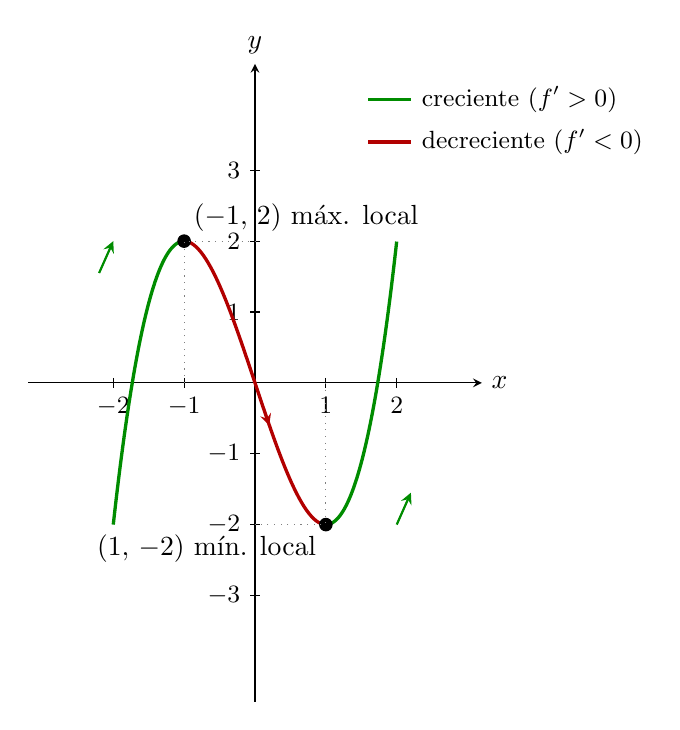
\begin{tikzpicture}[>=stealth, scale=0.9]

  % --- Ejes ---
  \draw[->] (-3.2,0) -- (3.2,0) node[right] {$x$};
  \draw[->] (0,-4.5) -- (0,4.5) node[above] {$y$};

  % --- Marcas en el eje x ---
  \foreach \x in {-2,-1,1,2}
    \draw (\x,0.07) -- (\x,-0.07) node[below, font=\small] {$\x$};

  % --- Marcas en el eje y ---
  \foreach \y in {-3,-2,-1,1,2,3}
    \draw (0.07,\y) -- (-0.07,\y) node[left, font=\small] {$\y$};

  % --- Curva f(x)=x^3-3x por tramos con color según monotonía ---
  % Tramo creciente: x in [-2, -1]  (verde)
  \draw[green!55!black, very thick, domain=-2:-1, samples=60]
        plot (\x, {\x*\x*\x - 3*\x});

  % Tramo decreciente: x in [-1, 1]  (red)
  \draw[red!70!black, very thick, domain=-1:1, samples=60]
        plot (\x, {\x*\x*\x - 3*\x});

  % Tramo creciente: x in [1, 2]  (verde)
  \draw[green!55!black, very thick, domain=1:2, samples=60]
        plot (\x, {\x*\x*\x - 3*\x});

  % --- Puntos críticos ---
  \filldraw[black] (-1, 2) circle (2.5pt)
        node[above right] {$(-1,\,2)$ máx. local};
  \filldraw[black] ( 1,-2) circle (2.5pt)
        node[below left]  {$(1,\,-2)$ mín. local};

  % --- Líneas de referencia punteadas ---
  \draw[dotted, gray] (-1,0) -- (-1,2) -- (0,2);
  \draw[dotted, gray] ( 1,0) -- ( 1,-2) -- (0,-2);

  % --- Flechas de monotonía sobre la curva ---
  % Creciente izquierda
  \draw[->, green!55!black, thick] (-2.2, 1.55) -- (-2.0, 2.0);
  % Decreciente centro
  \draw[->, red!70!black,   thick] (-0.2, 0.6)  -- ( 0.2,-0.6);
  % Creciente derecha
  \draw[->, green!55!black, thick] ( 2.0,-2.0)  -- ( 2.2,-1.55);

  % --- Leyenda ---
  \draw[green!55!black, very thick] (1.6, 4.0) -- (2.2, 4.0)
        node[right, black, font=\small] {creciente ($f'>0$)};
  \draw[red!70!black,   very thick] (1.6, 3.4) -- (2.2, 3.4)
        node[right, black, font=\small] {decreciente ($f'<0$)};

\end{tikzpicture}
\caption{Monotonía de $f(x)=x^3-3x$: la curva se colorea según el signo
de $f'$.}
\label{fig:monotonia_x3}
\end{figure}
\end{myproof}
\end{example}


La \textbf{concavidad} describe hacia qué lado «abre» la curva de $f$
en cada intervalo: como una taza ($\smile$) o como una cúpula ($\frown$).
Geométricamente, una figura es \emph{convexa} si el segmento que une
cualquier par de puntos interiores permanece dentro de ella, y
\emph{cóncava} en caso contrario. En el análisis de funciones, este
comportamiento lo detecta la segunda derivada: su signo indica si la
pendiente $f'$ crece o decrece a medida que $x$ avanza.

\begin{definition}
La gráfica de $f$ es \textbf{cóncava hacia arriba} en $(a,b)$ si $f'$
es creciente en ese intervalo, y \textbf{cóncava hacia abajo} si $f'$
es decreciente. Equivalentemente:
\[
f''(x)>0 \implies \text{cóncava hacia arriba}, \qquad
f''(x)<0 \implies \text{cóncava hacia abajo}.
\]
Un punto $c$ es un \textbf{punto de inflexión} de $f$ si $f$ es continua
en $c$ y la concavidad cambia de signo en $c$.
\end{definition}

\begin{rem}
Un punto donde $f''(c)=0$ no es necesariamente un punto de inflexión:
se requiere que $f''$ \emph{cambie de signo} en $c$. La función
$f(x)=x^4$ satisface $f''(0)=0$, pero la concavidad no cambia en $x=0$
(es cóncava hacia arriba en todo $\R$), por lo que $x=0$ no es punto de
inflexión.
\end{rem}

% ============================================================
\begin{example}[Concavidad e inflexiones de $f(x)=x^4-4x^3$]
Determinar los intervalos de concavidad y los puntos de inflexión de
$f(x)=x^4-4x^3$.
\begin{myproof}
\textbf{Paso 1. Calcular $f''$ y encontrar los puntos candidatos a
inflexión.}


\(
f'(x)  = 4x^3-12x^2, \qquad
f''(x) = 12x^2-24x  = 12x(x-2).
\)
Los ceros de $f''$ son los candidatos a puntos de inflexión: \(
12x(x-2)=0 \implies x=0 \quad\text{o}\quad x=2.
\)
Estos valores dividen la recta real en tres intervalos:
$(-\infty,0)$, $(0,2)$ y $(2,+\infty)$.

\textbf{Paso 2. Analizar el signo de $f''$ en cada intervalo.}

\begin{center}
\begin{tabular}{c c c c c}
\toprule
Intervalo & Signo de $12x$ & Signo de $(x-2)$ & Signo de $f''(x)$
& Concavidad \\
\midrule
$(-\infty,0)$ & $-$ & $-$ & $+$ & hacia arriba $\smile$ \\
$(0,\;2)$     & $+$ & $-$ & $-$ & hacia abajo  $\frown$ \\
$(2,+\infty)$ & $+$ & $+$ & $+$ & hacia arriba $\smile$ \\
\bottomrule
\end{tabular}
\end{center}

\textbf{Paso 3. Identificar los puntos de inflexión.}

En $x=0$ y $x=2$ la concavidad cambia de signo, por lo que ambos son
puntos de inflexión. Sus imágenes son: \(
f(0)=0, \qquad f(2)=16-32=-16.
\) Los puntos de inflexión son $(0,\,0)$ y $(2,\,-16)$.
\[
\boxed{\text{Inflexiones: }(0,0)\text{ y }(2,-16);\quad f''>0\text{ en }(-\infty,0)\cup(2,+\infty);\quad f''<0\text{ en }(0,2).}
\]

% ============================================================
% GRÁFICA: Concavidad de f(x) = x^4 - 4x^3
% ============================================================
\begin{figure}[H]
\centering
% ============================================================
% AJUSTE DE PROPORCIONES:
%   xscale → controla el ancho  (súbelo para más ancho)
%   yscale → controla el alto   (bájalo para menos alto)
%   Relación actual ≈ 2:1  (xscale=1.1, yscale=0.45)
% ============================================================
\begin{tikzpicture}[>=stealth, xscale=2.5, yscale=0.5]

  % --- Ejes ---
  \draw[->] (-1.5,0) -- (4.5,0) node[right] {$x$};
  \draw[->] (0,-18)  -- (0,6)   node[above] {$y$};

  % --- Marcas eje x ---
  \foreach \x in {-1,1,2,3,4}
    \draw (\x,0.25) -- (\x,-0.25) node[below, font=\small] {$\x$};

  % --- Marcas eje y ---
  \foreach \y in {-15,-10,-5,5}
    \draw (0.15,\y) -- (-0.15,\y) node[left, font=\small] {$\y$};

  % --- Curva por tramos coloreados según concavidad ---
  % Cóncava arriba: x in [-1.2, 0]
  \draw[blue!70!black, very thick, domain=-1:0, samples=60]
    plot (\x, {\x*\x*\x*\x - 4*\x*\x*\x});

  % Cóncava abajo: x in [0, 2]
  \draw[red!70!black, very thick, domain=0:2, samples=60]
    plot (\x, {\x*\x*\x*\x - 4*\x*\x*\x});

  % Cóncava arriba: x in [2, 4.2]
  \draw[blue!70!black, very thick, domain=2:3.5, samples=80]
    plot (\x, {\x*\x*\x*\x - 4*\x*\x*\x});

  % --- Puntos de inflexión ---
  % NOTA: circle necesita un radio proporcional; con escalas distintas
  % se usa "circle[radius=...]" para que no quede elipse
  \filldraw[black] (0,  0) circle[radius=3pt]
    node[above right, font=\small] {$(0,\,0)$ infl.};
  \filldraw[black] (2,-16) circle[radius=3pt]
    node[right, font=\small] {$(2,\,-16)$ infl.};

  % --- Líneas de referencia punteadas ---
  \draw[dotted, gray] (2,0) -- (2,-16) -- (0,-16);
  \node[left, font=\small, gray] at (0,-16) {$-16$};

  % --- Anotaciones de concavidad ---
  \node[blue!70!black, font=\small] at (-0.7,  4.5) {$f''>0$};
  \node[red!70!black,  font=\small] at ( 1.0, -5.5) {$f''<0$};
  \node[blue!70!black, font=\small] at ( 3.6, -5.0) {$f''>0$};

  % --- Símbolos de curvatura ---
  \node[blue!70!black] at (-0.6,  2.5) {$\smile$};
  \node[red!70!black]  at ( 1.0, -9.0) {$\frown$};
  \node[blue!70!black] at ( 3.5,-10.0) {$\smile$};

  % --- Leyenda ---
  \draw[blue!70!black, very thick] (2.8, 5.5) -- (3.3, 5.5)
    node[right, black, font=\small] {cóncava hacia arriba ($f''>0$)};
  \draw[red!70!black,  very thick] (2.8, 4.0) -- (3.3, 4.0)
    node[right, black, font=\small] {cóncava hacia abajo ($f''<0$)};

\end{tikzpicture}
\caption{Concavidad de $f(x)=x^4-4x^3$: en azul los tramos donde
$f''>0$ (curva abre hacia arriba) y en rojo donde $f''<0$ (curva abre
hacia abajo). Los puntos negros señalan los puntos de inflexión.}
\label{fig:concavidad_x4}
\end{figure}
\end{myproof}
\end{example}
Las herramientas desarrolladas hasta ahora de monotonía y concavidad
permiten caracterizar puntos especiales que son máximos o mínimos, no
en el dominio completo de $f$, sino en una vecindad reducida alrededor
de un punto. Estos se denominan \textbf{extremos locales} y representan
los \textit{picos} y \textit{valles} de la gráfica. Su localización se apoya en los
puntos críticos y puede abordarse mediante dos criterios: uno basado en
el cambio de signo de $f'$ y otro, más ágil cuando es aplicable, basado
en el signo de $f''$.

\begin{definition}
$f(c)$ es un \textbf{máximo local} si existe un intervalo abierto
$(a,b)$ que contiene a $c$ tal que $f(c)\geq f(x)$ para todo
$x\in(a,b)$. Análogamente se define el \textbf{mínimo local}.
\end{definition}

\begin{theorem}[Criterio de la primera derivada]
Sea $c$ un punto crítico de $f$:
\begin{itemize}
    \item Si $f'$ cambia de $+$ a $-$ en $c$: \textbf{máximo local}.
    \item Si $f'$ cambia de $-$ a $+$ en $c$: \textbf{mínimo local}.
    \item Si $f'$ no cambia de signo en $c$: no hay extremo local.
\end{itemize}
\end{theorem}

\begin{theorem}[Criterio de la segunda derivada]
Si $f'(c)=0$ y $f''(c)$ existe:
\begin{itemize}
    \item $f''(c)<0$: \textbf{máximo local} (la curva es cóncava hacia
    abajo en $c$).
    \item $f''(c)>0$: \textbf{mínimo local} (la curva es cóncava hacia
    arriba en $c$).
    \item $f''(c)=0$: el criterio es \textbf{inconcluso}; puede haber
    máximo, mínimo o punto de inflexión.
\end{itemize}
\end{theorem}

\begin{rem}
El caso $f''(c)=0$ ilustra la importancia de no abandonar el análisis
prematuramente. Para $f(x)=x^4$, se tiene $f'(0)=0$ y $f''(0)=0$,
pero $x=0$ es un mínimo local; para $f(x)=x^3$, las mismas condiciones
se cumplen en $x=0$, pero se trata de un punto de inflexión. El criterio
de la segunda derivada no distingue estos casos, por lo que siempre debe
recurrirse al de la primera derivada cuando $f''(c)=0$.
\end{rem}

\begin{example}[Análisis completo de $f(x)=x^4-4x^3$]
Analizar completamente $f(x)=x^4-4x^3$.
\begin{myproof}
\textbf{Paso 1. Dominio e información básica.}

$f$ es un polinomio, por lo que su dominio es $\mathbb{R}$, es continua
y derivable en todo punto. Como el término dominante es $x^4>0$, la
función tiende a $+\infty$ en ambos extremos.

\textbf{Paso 2. Puntos críticos y monotonía.}

Se calcula la primera derivada y se factoriza:
\[
f'(x) = 4x^3 - 12x^2 = 4x^2(x-3).
\]
Los puntos críticos, donde $f'(x)=0$, son $x=0$ y $x=3$. Estos dos
valores dividen la recta real en tres intervalos. Se analiza el signo
de cada factor en cada uno de ellos:

\begin{center}
\begin{tabular}{c c c c c}
\toprule
Intervalo & Signo de $4x^2$ & Signo de $(x-3)$ & Signo de $f'(x)$
& Monotonía \\
\midrule
$(-\infty,\,0)$ & $+$ & $-$ & $-$ & decreciente \\
$(0,\,3)$       & $+$ & $-$ & $-$ & decreciente \\
$(3,\,+\infty)$ & $+$ & $+$ & $+$ & creciente   \\
\bottomrule
\end{tabular}
\end{center}

Nótese que $f'$ mantiene el signo negativo a ambos lados de $x=0$: la
función sigue decreciendo sin interrupciones al pasar por ese punto, de
modo que \textbf{no hay extremo local en $x=0$}. En cambio, en $x=3$
la derivada cambia de $-$ a $+$, lo que por el criterio de la primera
derivada confirma un \textbf{mínimo local}:
\[
f(3) = 81 - 108 = -27.
\]

\textbf{Paso 3. Concavidad y puntos de inflexión.}

Se calcula la segunda derivada:
\[
f''(x) = 12x^2 - 24x = 12x(x-2).
\]
Los candidatos a puntos de inflexión son $x=0$ y $x=2$. Se analiza el
signo de $f''$ en los tres intervalos resultantes:

\begin{center}
\begin{tabular}{c c c c c}
\toprule
Intervalo & Signo de $12x$ & Signo de $(x-2)$ & Signo de $f''(x)$
& Concavidad \\
\midrule
$(-\infty,\,0)$ & $-$ & $-$ & $+$ & hacia arriba $\smile$ \\
$(0,\,2)$       & $+$ & $-$ & $-$ & hacia abajo  $\frown$ \\
$(2,\,+\infty)$ & $+$ & $+$ & $+$ & hacia arriba $\smile$ \\
\bottomrule
\end{tabular}
\end{center}

Como $f''$ cambia de signo en $x=0$ (de $+$ a $-$) y en $x=2$ (de $-$
a $+$), ambos son \textbf{puntos de inflexión}. Sus imágenes son:
\[
f(0) = 0, \qquad f(2) = 16 - 32 = -16.
\]

Se puede aplicar también el criterio de la segunda derivada en $x=3$
para confirmar el mínimo: $f''(3)=12(3)(1)=36>0$, lo que indica
concavidad hacia arriba, consistente con un mínimo local. En $x=0$,
en cambio, $f''(0)=0$, por lo que el criterio de la segunda derivada
es inconcluso allí; fue el análisis de la primera derivada el que
permitió concluir que no hay extremo en ese punto.

\textbf{Resumen del análisis completo.}

\begin{center}
\begin{tabular}{c l}
\toprule
Punto & Clasificación \\
\midrule
$x=0$ & Punto de inflexión en $(0,\,0)$; no es extremo local. \\
$x=2$ & Punto de inflexión en $(2,\,-16)$. \\
$x=3$ & Mínimo local en $(3,\,-27)$. \\
\bottomrule
\end{tabular}
\end{center}

La función decrece en $(-\infty,3)$, alcanza su único mínimo local en
$x=3$, y crece en $(3,+\infty)$. La concavidad cambia en $x=0$ y
$x=2$, que son los únicos puntos de inflexión.
\[
\boxed{\text{Mínimo local: }(3,-27);\quad\text{inflexiones: }(0,0)\text{ y }(2,-16).}
\]
El bosquejo de la función puede revisarse nuevamente en la figura \ref{fig:concavidad_x4}.
\end{myproof}
\end{example}

%%==========================================================
\section{Trazado Sistemático de Curvas}
%%==========================================================

El análisis desarrollado en las secciones anteriores no es un fin en sí
mismo: monotonía, concavidad, extremos locales y puntos de inflexión son
piezas de un mismo rompecabezas cuyo resultado final es la comprensión
global del comportamiento de una función. Reunir todas estas herramientas
en un procedimiento ordenado permite \textbf{bosquejar la gráfica de
cualquier función} de manera rigurosa, sin depender de tablas de valores
construidas punto a punto. La ventaja de este enfoque es doble: por un
lado, la gráfica resultante refleja fielmente la estructura matemática de
$f$; por el otro, el proceso mismo de análisis obliga a comprender la
función antes de representarla. El protocolo que se presenta a
continuación organiza ese proceso en cuatro etapas progresivas, donde
cada paso alimenta al siguiente.

\begin{pasos}
Para bosquejar la gráfica de una función es posible seguir el siguiente
proceso sistemático:
\begin{enumerate}
    \item \textbf{Análisis previo.} Determinar dominio, rango (si es
    posible), simetría (par/impar/periódica), intersecciones con los
    ejes y comportamiento asintótico ($x\to\pm\infty$, puntos
    singulares).
    \item \textbf{Primera derivada.} Calcular $f'$, hallar puntos
    críticos, determinar intervalos de crecimiento y decrecimiento,
    clasificar extremos locales.
    \item \textbf{Segunda derivada.} Calcular $f''$, determinar
    intervalos de concavidad y localizar puntos de inflexión.
    \item \textbf{Tabla y bosquejo.} Resumir toda la información en
    una tabla de puntos clave. Trazar primero las asíntotas, luego
    los puntos especiales, y conectarlos respetando la monotonía y la
    concavidad.
\end{enumerate}
\end{pasos}

\begin{example}[Trazado de $f(x)=x^2/(x^2-4)$]
Trazar la curva $f(x)=\dfrac{x^2}{x^2-4}$.
\begin{myproof}
\textbf{Paso 1. Análisis previo.}

\emph{Dominio.} El denominador $x^2-4=(x-2)(x+2)$ se anula en $x=\pm2$,
de modo que el dominio es $\mathbb{R}\setminus\{-2,\,2\}$.

\emph{Simetría.} Como $f(-x)=\dfrac{(-x)^2}{(-x)^2-4}=\dfrac{x^2}{x^2-4}=f(x)$,
la función es \textbf{par}: su gráfica es simétrica respecto al eje $y$.
Esto permite analizar $x\geq 0$ y reflejar.

\emph{Intersecciones.} En $x=0$: $f(0)=0$, luego la curva pasa por el
origen. La ecuación $f(x)=0$ implica $x^2=0$, es decir, $x=0$ es la
única intersección con ambos ejes.

\emph{Asíntotas verticales.} En $x=2$ y $x=-2$ el denominador se anula
y el numerador no, por lo que existen asíntotas verticales en ambos
puntos. Analizando los límites laterales en $x=2$:
\[
\lim_{x\to 2^-}f(x)=-\infty, \qquad \lim_{x\to 2^+}f(x)=+\infty,
\]
y por simetría los comportamientos en $x=-2$ son opuestos.

\emph{Asíntota horizontal.} Dividiendo numerador y denominador entre
$x^2$:
\[
\lim_{x\to\pm\infty}f(x)=\lim_{x\to\pm\infty}\frac{1}{1-4/x^2}=1,
\]
de modo que $y=1$ es asíntota horizontal. Nótese además que $f(x)=1$
no tiene solución ($x^2=x^2-4$ es imposible), así que la curva nunca
toca su propia asíntota horizontal.

\textbf{Paso 2. Primera derivada: monotonía y extremos locales.}

Aplicando la regla del cociente:
\[
f'(x)
= \frac{2x(x^2-4)-x^2\cdot 2x}{(x^2-4)^2}
= \frac{2x^3-8x-2x^3}{(x^2-4)^2}
= \frac{-8x}{(x^2-4)^2}.
\]
El único punto crítico interior al dominio es $x=0$, pues $f'(x)=0$
implica $x=0$. Como $(x^2-4)^2>0$ siempre, el signo de $f'$ queda
determinado únicamente por $-8x$:

\begin{center}
\begin{tabular}{c c c}
\toprule
Intervalo & Signo de $f'(x)$ & Monotonía \\
\midrule
$(-\infty,-2)$ & $+$ & creciente \\
$(-2,\;0)$     & $+$ & creciente \\
$(0,\;2)$      & $-$ & decreciente \\
$(2,+\infty)$  & $-$ & decreciente \\
\bottomrule
\end{tabular}
\end{center}

En $x=0$ la derivada cambia de $+$ a $-$, lo que indica un
\textbf{máximo local} con valor $f(0)=0$. Obsérvese que, aunque la
función crece en $(-\infty,-2)$ y en $(-2,0)$, estos son intervalos
separados por la discontinuidad en $x=-2$; no se puede afirmar que $f$
crece en $(-\infty,0)$ en su conjunto.

\textbf{Paso 3. Segunda derivada: concavidad y puntos de inflexión.}

Derivando $f'(x)=\dfrac{-8x}{(x^2-4)^2}$ mediante la regla del cociente:
\[
f''(x)
= \frac{-8(x^2-4)^2 - (-8x)\cdot 2(x^2-4)\cdot 2x}{(x^2-4)^4}
= \frac{-8(x^2-4)+32x^2}{(x^2-4)^3}
= \frac{8(3x^2+4)}{(x^2-4)^3}.
\]
El numerador $8(3x^2+4)>0$ para todo $x\in\mathbb{R}$, de modo que el
signo de $f''$ depende exclusivamente del denominador $(x^2-4)^3$:

\begin{center}
\begin{tabular}{c c c c}
\toprule
Intervalo & Signo de $(x^2-4)^3$ & Signo de $f''(x)$ & Concavidad \\
\midrule
$(-\infty,-2)$ & $+$ & $+$ & hacia arriba $\smile$ \\
$(-2,\;2)$     & $-$ & $-$ & hacia abajo  $\frown$ \\
$(2,+\infty)$  & $+$ & $+$ & hacia arriba $\smile$ \\
\bottomrule
\end{tabular}
\end{center}

Como $f''(x)=0$ no tiene solución real, \textbf{no hay puntos de
inflexión}. La concavidad cambia únicamente en las asíntotas verticales,
que no pertenecen al dominio.

\textbf{Paso 4. Tabla resumen y bosquejo.}

\begin{center}
\renewcommand{\arraystretch}{1.3}
\begin{tabular}{c c c c}
\toprule
Intervalo & $f'$ & $f''$ & Comportamiento \\
\midrule
$(-\infty,-2)$ & $+$ & $+$ & creciente, cóncava $\uparrow$ \\
$(-2,\;0)$     & $+$ & $-$ & creciente, cóncava $\downarrow$ \\
$(0,\;2)$      & $-$ & $-$ & decreciente, cóncava $\downarrow$ \\
$(2,+\infty)$  & $-$ & $+$ & decreciente, cóncava $\uparrow$ \\
\bottomrule
\end{tabular}
\end{center}

\[
\boxed{\text{Máx. local: }(0,0);\quad\text{asíntotas verticales: }x=\pm2;\quad\text{asíntota horizontal: }y=1.}
\]

% ============================================================
% BOSQUEJO: f(x) = x^2 / (x^2 - 4)
% ============================================================
\begin{figure}[H]
\centering
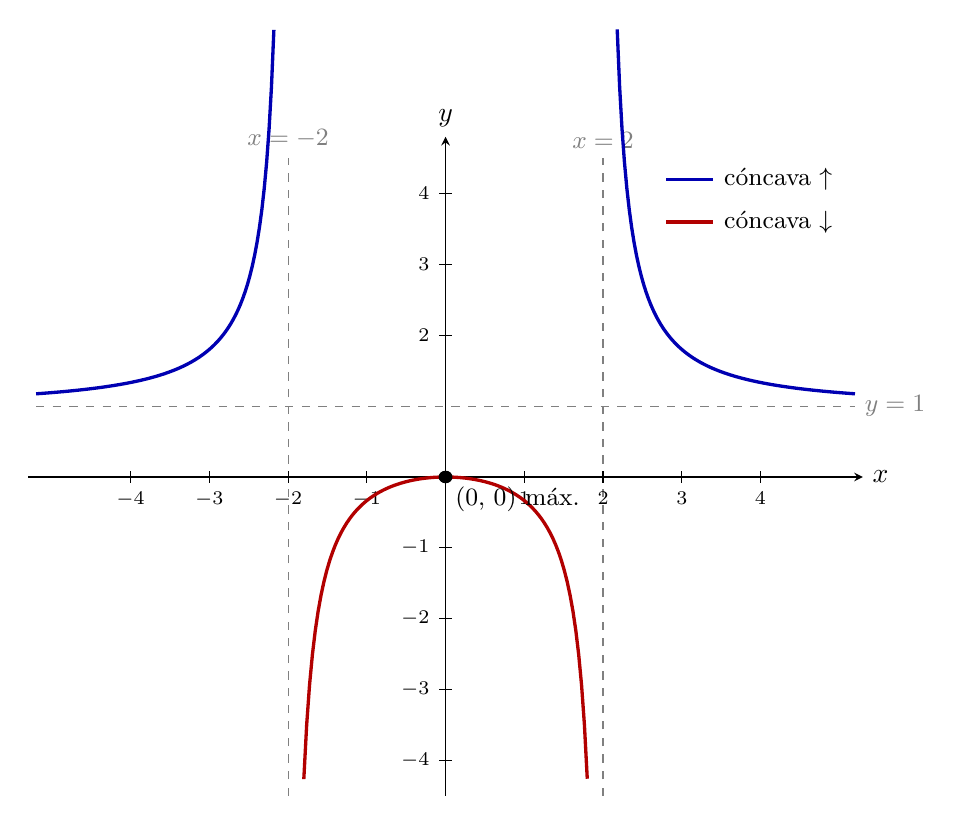
\begin{tikzpicture}[>=stealth, xscale=1.0, yscale=0.9]

  % --- Asíntotas ---
  \draw[gray, dashed, thin] (-2,-4.5) -- (-2, 4.5)
        node[above, font=\small] {$x=-2$};
  \draw[gray, dashed, thin] ( 2,-4.5) -- ( 2, 4.5)
        node[above, font=\small] {$x=2$};
  \draw[gray, dashed, thin] (-5.2, 1) -- ( 5.2, 1)
        node[right, font=\small] {$y=1$};

  % --- Ejes ---
  \draw[->] (-5.3,0) -- (5.3,0) node[right] {$x$};
  \draw[->] (0,-4.5) -- (0,4.8) node[above] {$y$};

  % --- Marcas eje x ---
  \foreach \x in {-4,-3,-2,-1,1,2,3,4}
    \draw (\x,0.08) -- (\x,-0.08)
          node[below, font=\scriptsize] {$\x$};

  % --- Marcas eje y ---
  \foreach \y in {-4,-3,-2,-1,2,3,4}
    \draw (0.08,\y) -- (-0.08,\y)
          node[left, font=\scriptsize] {$\y$};

  % --- Rama izquierda: x in (-inf, -2)  -> creciente, cóncava arriba ---
  \draw[blue!70!black, very thick, domain=-5.2:-2.18, samples=100]
    plot (\x, {\x*\x/(\x*\x-4)});

  % --- Rama central: x in (-2, 2)  -> cóncava abajo, máx en (0,0) ---
  \draw[red!70!black, very thick, domain=-1.8:1.8, samples=100]
    plot (\x, {\x*\x/(\x*\x-4)});

  % --- Rama derecha: x in (2, inf)  -> decreciente, cóncava arriba ---
  \draw[blue!70!black, very thick, domain=2.18:5.2, samples=100]
    plot (\x, {\x*\x/(\x*\x-4)});

  % --- Máximo local en (0,0) ---
  \filldraw[black] (0,0) circle[radius=2.3pt]
    node[below right, font=\small] {$(0,\,0)$ máx.};

  % --- Leyenda ---
  \draw[blue!70!black, very thick] (2.8, 4.2) -- (3.4, 4.2)
    node[right, black, font=\small] {cóncava $\uparrow$};
  \draw[red!70!black,  very thick] (2.8, 3.6) -- (3.4, 3.6)
    node[right, black, font=\small] {cóncava $\downarrow$};

\end{tikzpicture}
\caption{Bosquejo de $f(x)=\dfrac{x^2}{x^2-4}$. Las ramas azules son
cóncavas hacia arriba y las rojas hacia abajo. Las líneas grises
punteadas indican las asíntotas $x=\pm2$ e $y=1$.}
\label{fig:bosquejo_racional}
\end{figure}
\end{myproof}
\end{example}
%%%==========================================================
\section{Optimización}
%%==========================================================

El trazado sistemático de curvas muestra que el cálculo diferencial
permite entender el comportamiento global de una función: dónde crece,
dónde decrece, dónde alcanza sus picos y valles. Este mismo aparato
puede orientarse hacia una pregunta de enorme utilidad práctica:
¿cuál es el \emph{mejor} valor posible de una cantidad? Diseñar un
envase con el menor material posible, determinar el precio que maximiza
los ingresos de una empresa, o encontrar la trayectoria de menor tiempo
entre dos puntos son problemas que, en apariencia, pertenecen a dominios
muy distintos. Sin embargo, todos comparten la misma estructura
matemática: existe una \textbf{función objetivo} que se desea maximizar
o minimizar, y una o varias \textbf{restricciones} que acotan los
valores admisibles de las variables. El cálculo diferencial resuelve
esta clase de problemas de forma exacta, localizando los puntos críticos
de la función objetivo y clasificándolos mediante los criterios de la
primera o la segunda derivada. El procedimiento sistemático es el
siguiente.

\begin{pasos}
El siguiente es un procedimiento sistemático para resolver problemas
de optimización:
\begin{enumerate}
    \item \textbf{Diagrama y variables.} Asignar símbolos a todas las
    cantidades relevantes y realizar un diagrama representativo.
    \item \textbf{Función objetivo.} Escribir la fórmula de la cantidad
    $Q$ que se desea optimizar.
    \item \textbf{Reducción a una variable.} Usar las restricciones para
    expresar $Q$ en función de una sola variable y determinar su dominio.
    \item \textbf{Localizar puntos críticos.} Resolver $\dfrac{dQ}{dx}=0$
    y verificar singularidades o extremos del dominio.
    \item \textbf{Clasificar el extremo.} Usar el criterio de la primera
    o segunda derivada para confirmar que se trata de un máximo o mínimo.
\end{enumerate}
\end{pasos}



% ============================================================
\begin{example}[Caja abierta de volumen máximo]
De una hoja rectangular de $24\times 9$ cm se recortan cuadrados
iguales en las esquinas y se doblan los bordes para formar una caja
abierta. ¿Qué tamaño deben tener los cuadrados para maximizar el
volumen?
\begin{myproof}
\textbf{Paso 1. Diagrama y variables.}

Sea $x$ el lado (en cm) de cada cuadrado recortado en las esquinas.
Al doblar los bordes, la caja resultante tiene:
base de $(24-2x)\times(9-2x)$ cm y altura $x$ cm.

\begin{figure}[H]
\centering
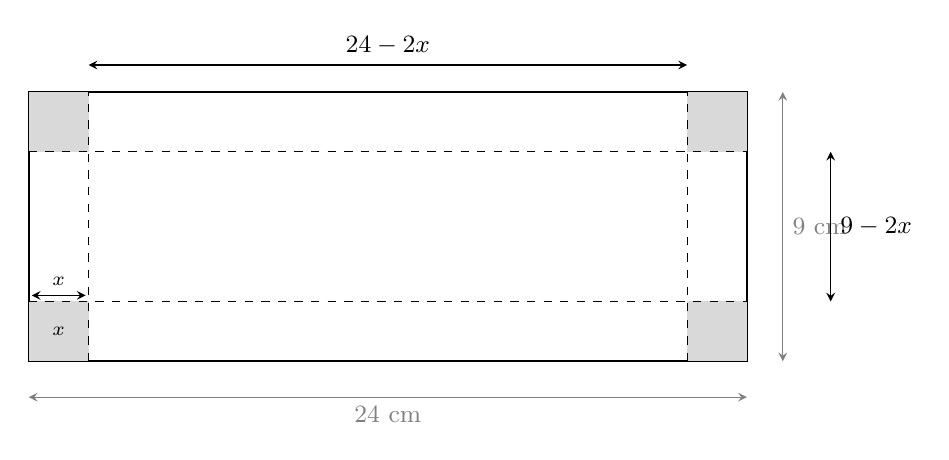
\begin{tikzpicture}[>=stealth, xscale=0.38, yscale=0.38]
  % Hoja completa
  \draw[thick] (0,0) rectangle (24,9);

  % Cuadrados recortados (sombreados)
  \fill[gray!30] (0,0)  rectangle (2,2);
  \fill[gray!30] (22,0) rectangle (24,2);
  \fill[gray!30] (0,7)  rectangle (2,9);
  \fill[gray!30] (22,7) rectangle (24,9);

  % Bordes de los cuadrados
  \draw[dashed] (2,0)--(2,9);
  \draw[dashed] (22,0)--(22,9);
  \draw[dashed] (0,2)--(24,2);
  \draw[dashed] (0,7)--(24,7);

  % Cotas externas
  \draw[<->, gray] (0,-1.2) -- (24,-1.2)
        node[midway, below, font=\small] {$24$ cm};
  \draw[<->, gray] (25.2,0) -- (25.2,9)
        node[midway, right, font=\small] {$9$ cm};

  % Cotas internas
  \draw[<->] (2,9.9) -- (22,9.9)
        node[midway, above, font=\small] {$24-2x$};
  \draw[<->] (26.8,2) -- (26.8,7)
        node[midway, right, font=\small] {$9-2x$};
  \draw[<->] (0.1,2.2) -- (1.9,2.2)
        node[midway, above, font=\scriptsize] {$x$};

  % Etiqueta cuadrado
  \node[font=\scriptsize] at (1,1) {$x$};
\end{tikzpicture}
\hspace{1.5cm}
% Caja 3D
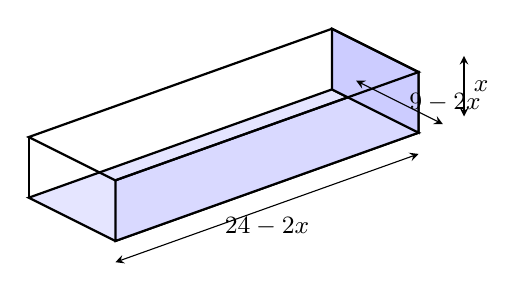
\begin{tikzpicture}[>=stealth,
    x={(0.7cm,0.25cm)}, y={(0cm,0.7cm)}, z={(-0.4cm,0.2cm)},
    scale=0.55]
  % Base
  \draw[thick,fill=blue!10]
    (0,0,0)--(10,0,0)--(10,0,5)--(0,0,5)--cycle;
  % Frente
  \draw[thick,fill=blue!15]
    (0,0,0)--(10,0,0)--(10,2,0)--(0,2,0)--cycle;
  % Lado derecho
  \draw[thick,fill=blue!20]
    (10,0,0)--(10,0,5)--(10,2,5)--(10,2,0)--cycle;
  % Aristas superiores
  \draw[thick]
    (0,2,0)--(10,2,0)--(10,2,5)--(0,2,5)--(0,2,0);
  \draw[thick] (0,0,5)--(0,2,5);

  % Cotas
  \draw[<->] (0,-0.7,0)--(10,-0.7,0)
        node[midway,below,font=\small]{$24-2x$};
  \draw[<->] (10.8,0,0)--(10.8,0,5)
        node[midway,right,font=\small]{$9-2x$};
  \draw[<->] (11.5,0,0)--(11.5,2,0)
        node[midway,right,font=\small]{$x$};
\end{tikzpicture}
\caption{Construcción de la caja abierta: se recortan cuadrados de lado $x$
  en las esquinas de la lámina de $24\times 9$ cm y se doblan los bordes,
  quedando una base de $(24-2x)\times(9-2x)$ y altura $x$.}
\label{fig:caja_abierta_recorte}
\end{figure}

\textbf{Paso 2. Función objetivo.}

La cantidad a maximizar es el volumen de la caja:
\[
V = \text{base} \times \text{altura}
  = (24-2x)(9-2x)\cdot x.
\]

\textbf{Paso 3. Reducción a una variable y dominio.}

Expandiendo el producto:
\[
V(x) = x(24-2x)(9-2x)
      = x\bigl(216 - 48x - 18x + 4x^2\bigr)
      = 4x^3 - 66x^2 + 216x.
\]
Para que la caja exista se necesita $x>0$ y $9-2x>0$, de modo que
el dominio es $x\in\!\left(0,\,\tfrac{9}{2}\right)$.

\textbf{Paso 4. Localizar puntos críticos.}

\[
V'(x) = 12x^2 - 132x + 216 = 12(x^2 - 11x + 18) = 12(x-2)(x-9).
\]
Las raíces son $x=2$ y $x=9$. Como $x=9\notin\!\left(0,\tfrac{9}{2}\right)$,
el único punto crítico interior es $\boldsymbol{x=2}$.

\textbf{Paso 5. Clasificar el extremo.}

Se aplica el criterio de la segunda derivada:
\[
V''(x) = 24x - 132 \implies V''(2) = 48 - 132 = -84 < 0.
\]
El signo negativo confirma un \textbf{máximo local} en $x=2$.
Comparando con los extremos del dominio, donde $V(0)=V\!\left(\tfrac{9}{2}\right)=0$,
se concluye que $x=2$ produce el \textbf{máximo absoluto} en el
intervalo. El volumen máximo es:
\[
V(2) = 2(24-4)(9-4) = 2\cdot 20\cdot 5 = \boxed{200 \text{ cm}^3}.
\]
Los cuadrados deben tener \textbf{2 cm de lado}.
\end{myproof}
\end{example}


% ============================================================
\begin{example}[Lata cilíndrica sin tapa de área mínima]
Se desea construir una lata cilíndrica sin tapa de volumen $V_0$.
Encontrar las dimensiones que minimizan el área total de material
utilizado.
\begin{myproof}
\textbf{Paso 1. Diagrama y variables.}

Sean $r$ el radio de la base y $h$ la altura del cilindro.

\begin{figure}[H]
\centering
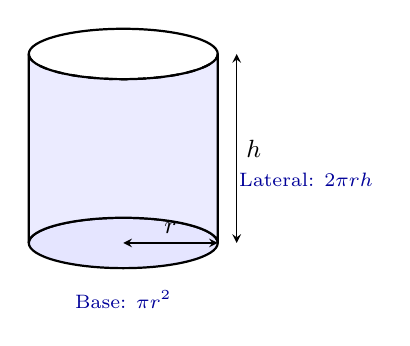
\begin{tikzpicture}[>=stealth, scale=0.8]
  % Cilindro abierto
  % Base inferior (elipse)
  \draw[thick, fill=blue!10]
    (0,0) ellipse (1.5 and 0.4);
  % Paredes laterales
  \draw[thick, fill=blue!8]
    (-1.5,0) -- (-1.5,3) arc(180:360:1.5 and 0.4) -- (1.5,0)
    arc(0:180:1.5 and 0.4);
  % Borde superior (abierto)
  \draw[thick, dashed] (-1.5,3) arc(180:360:1.5 and 0.4);
  \draw[thick] (-1.5,3) arc(180:0:1.5 and 0.4);

  % Cota radio
  \draw[<->] (0,0) -- (1.5,0)
        node[midway, above, font=\small] {$r$};
  % Cota altura
  \draw[<->] (1.8,0) -- (1.8,3)
        node[midway, right, font=\small] {$h$};

  % Etiquetas de áreas
  \node[font=\scriptsize, blue!60!black] at (0,-0.9)
        {Base: $\pi r^2$};
  \node[font=\scriptsize, blue!60!black] at (2.9,1)
        {Lateral: $2\pi r h$};
\end{tikzpicture}
\caption{Lata cilíndrica abierta de radio $r$ y altura $h$: el material total
  es el área de la base $\pi r^2$ más la pared lateral $2\pi r h$.}
\label{fig:lata_cilindrica}
\end{figure}

\textbf{Paso 2. Función objetivo.}

El área total de material (base circular más pared lateral) es:
\[
A = \pi r^2 + 2\pi r h.
\]

\textbf{Paso 3. Reducción a una variable y dominio.}

La restricción de volumen es $\pi r^2 h = V_0$, de donde
$h = \dfrac{V_0}{\pi r^2}$.
Sustituyendo en $A$:
\[
A(r) = \pi r^2 + 2\pi r \cdot \frac{V_0}{\pi r^2}
      = \pi r^2 + \frac{2V_0}{r}, \qquad r\in(0,+\infty).
\]

\textbf{Paso 4. Localizar puntos críticos.}

\[
A'(r) = 2\pi r - \frac{2V_0}{r^2} = 0
\implies 2\pi r = \frac{2V_0}{r^2}
\implies r^3 = \frac{V_0}{\pi}
\implies \boldsymbol{r = \left(\frac{V_0}{\pi}\right)^{1/3}}.
\]

\textbf{Paso 5. Clasificar el extremo.}

\[
A''(r) = 2\pi + \frac{4V_0}{r^3} > 0 \quad \text{para todo } r>0,
\]
lo que confirma un \textbf{mínimo}. La altura óptima vale:
\[
h = \frac{V_0}{\pi r^2}
  = \frac{\pi r^3}{\pi r^2} = r.
\]
La lata de menor material se obtiene cuando \textbf{la altura iguala
al radio}:
\[
\boxed{h = r = \left(\frac{V_0}{\pi}\right)^{1/3}.}
\]
\end{myproof}
\end{example}


% ============================================================
\begin{example}[Tendido de tubería a mínimo costo]
Una tubería debe ir desde el punto $A$ en una orilla de un río de
$3$ km de ancho hasta el punto $B$, situado $8$ km aguas abajo en la
orilla opuesta. Tender tubería por el río cuesta \$200/km y por
tierra \$100/km. ¿Dónde debe cruzar el río para minimizar el costo
total?
\begin{myproof}
\textbf{Paso 1. Diagrama y variables.}

Sea $C$ el punto de cruce en la orilla de $B$, y sea $x$ la distancia
horizontal desde el punto directamente opuesto a $A$ hasta $C$, con
$x\in[0,8]$.

\begin{figure}[H]
\centering
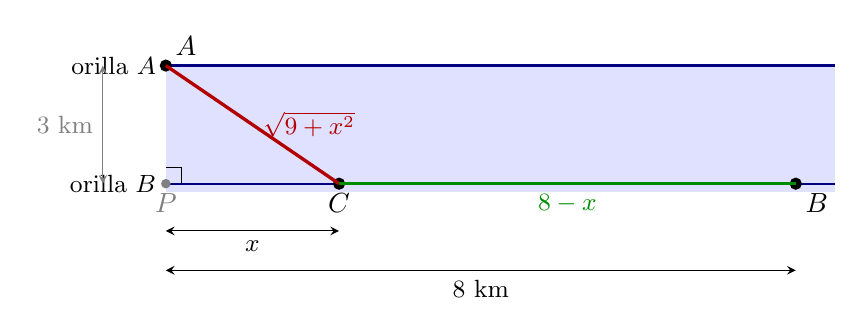
\begin{tikzpicture}[>=stealth, xscale=1.0, yscale=1.0]
  % Orillas del río
  \fill[blue!12] (0,-0.1) rectangle (8.5,1.5);
  \draw[blue!50!black, thick] (0,0)   -- (8.5,0);   % orilla inferior (B)
  \draw[blue!50!black, thick] (0,1.5) -- (8.5,1.5); % orilla superior (A)

  % Etiquetas orillas
  \node[left, font=\small] at (0,1.5) {orilla $A$};
  \node[left, font=\small] at (0,0)   {orilla $B$};

  % Punto A
  \filldraw[black] (0,1.5) circle (2pt) node[above right]{$A$};

  % Punto directamente opuesto a A
  \filldraw[gray]  (0,0)   circle (1.5pt) node[below]{$P$};

  % Punto C (cruce)
  \filldraw[black] (2.2,0) circle (2pt) node[below]{$C$};

  % Punto B
  \filldraw[black] (8,0)   circle (2pt) node[below right]{$B$};

  % Tubería submarina A -> C
  \draw[red!70!black, very thick] (0,1.5) -- (2.2,0)
        node[midway, right, font=\small]{$\sqrt{9+x^2}$};

  % Tubería terrestre C -> B
  \draw[green!55!black, very thick] (2.2,0) -- (8,0)
        node[midway, below, font=\small]{$8-x$};

  % Cota ancho río
  \draw[<->, gray] (-0.8,0) -- (-0.8,1.5)
        node[midway, left, font=\small]{$3$ km};

  % Cota x
  \draw[<->] (0,-0.6) -- (2.2,-0.6)
        node[midway, below, font=\small]{$x$};

  % Cota 8
  \draw[<->] (0,-1.1) -- (8,-1.1)
        node[midway, below, font=\small]{$8$ km};

  % Ángulo recto P
  \draw (0.2,0) -- (0.2,0.2) -- (0,0.2);
\end{tikzpicture}
\caption{Tendido de tubería: cruce del río (ancho $3$ km) desde $A$ hasta el
  punto $C$ a distancia $x$ de $P$, y tramo terrestre $C\to B$ de longitud
  $8-x$. El tramo submarino mide $\sqrt{9+x^2}$.}
\label{fig:tuberia_rio}
\end{figure}

\textbf{Paso 2. Función objetivo.}

El costo total combina el tramo subacuático $A\to C$ y el tramo
terrestre $C\to B$:
\[
\text{Costo}(x)
= 200\sqrt{9+x^2} + 100(8-x), \qquad x\in[0,8].
\]

\textbf{Paso 3. Reducción a una variable y dominio.}

La función ya depende de una sola variable $x$. El dominio es el
intervalo cerrado $[0,8]$, lo que garantiza la existencia del mínimo
absoluto por el Teorema del Valor Extremo.

\textbf{Paso 4. Localizar puntos críticos.}

\begin{align*}
\text{Costo}'(x)
= \frac{200x}{\sqrt{9+x^2}} - 100 = 0
&\implies \frac{2x}{\sqrt{9+x^2}} = 1\\
&\implies 4x^2 = 9+x^2\\
&\implies 3x^2 = 9
\implies x = \sqrt{3} \approx 1.73 \text{ km}.
\end{align*}
El valor negativo $x=-\sqrt{3}$ queda fuera del dominio y se descarta.

\textbf{Paso 5. Clasificar el extremo.}

\[
\text{Costo}''(x)
= \frac{200\cdot 9}{(9+x^2)^{3/2}} > 0
\quad \text{para todo } x\in[0,8],
\]
lo que confirma un \textbf{mínimo}. Comparando con los extremos del
intervalo:
\begin{align*}
\text{Costo}(0)      &= 200(3)+100(8) = 1400 \text{ USD}\\
\text{Costo}(8)      &= 200\sqrt{73}  \approx 1709 \text{ USD}\\
\text{Costo}(\sqrt{3}) &= 400\sqrt{3}+100(8-\sqrt{3}) = 300\sqrt{3}+800\approx \boxed{1319.6 \text{ USD}}.
\end{align*}
El cruce óptimo se ubica \textbf{a $\sqrt{3}\approx 1.73$ km} del
punto $P$ directamente opuesto a $A$, produciendo el costo mínimo
de aproximadamente $\$1319.6$ USD.
\end{myproof}
\end{example}
%%==========================================================
\section{El Teorema del Valor Medio}
%%==========================================================

Los criterios de monotonía y optimización desarrollados en las secciones
anteriores descansan sobre una garantía más profunda: si una función es
suficientemente regular en un intervalo, su derivada no puede comportarse
de forma arbitraria. El resultado que formaliza esta idea es el
\textbf{Teorema del Valor Medio}, uno de los teoremas más importantes
del cálculo diferencial. Su punto de partida es un caso particular
elemental, conocido como el Lema de Rolle, que captura una observación
geométrica sencilla: si una curva comienza y termina a la misma altura,
en algún punto intermedio debe ser horizontal.

\begin{lemma}[Rolle]
Si $f$ es continua en $[a,b]$, derivable en $(a,b)$ y $f(a)=f(b)$,
entonces existe al menos un $c\in(a,b)$ tal que $f'(c)=0$.
\end{lemma}

\begin{proof}[Esquema]
Por el Teorema del Valor Extremo de Weierstrass, $f$ alcanza en $[a,b]$ un
máximo y un mínimo absolutos. Si ambos se alcanzan en los extremos, entonces
$f$ es constante (pues $f(a)=f(b)$) y $f'(c)=0$ para todo $c\in(a,b)$. En caso
contrario, al menos uno de los dos extremos absolutos se alcanza en un punto
interior $c\in(a,b)$; siendo $f$ derivable allí, el Teorema de Fermat garantiza
que $f'(c)=0$.
\end{proof}

El Teorema del Valor Medio generaliza esta idea eliminando la exigencia
de que los extremos tengan la misma imagen: ahora se garantiza la
existencia de un punto donde la pendiente de la tangente coincide con
la pendiente de la recta que une los dos extremos de la curva.

\begin{theorem}[del Valor Medio de Lagrange]
Si $f$ es continua en $[a,b]$ y derivable en $(a,b)$, existe al menos
un $c\in(a,b)$ tal que
\[
f'(c) = \frac{f(b)-f(a)}{b-a}.
\]
\end{theorem}

Geométricamente, el TVM garantiza que existe un punto en la curva donde
la recta tangente es \textbf{paralela} a la recta secante que une los
extremos del intervalo. La interpretación física es igualmente
iluminadora: si un automóvil recorre $120$ km en $2$ horas (velocidad
promedio $60$ km/h), en algún instante exacto su velocidad instantánea
fue exactamente $60$ km/h. El siguiente ejemplo muestra que el TVM no
es un resultado independiente, sino una consecuencia directa del Lema
de Rolle.

\begin{figure}[H]
\centering
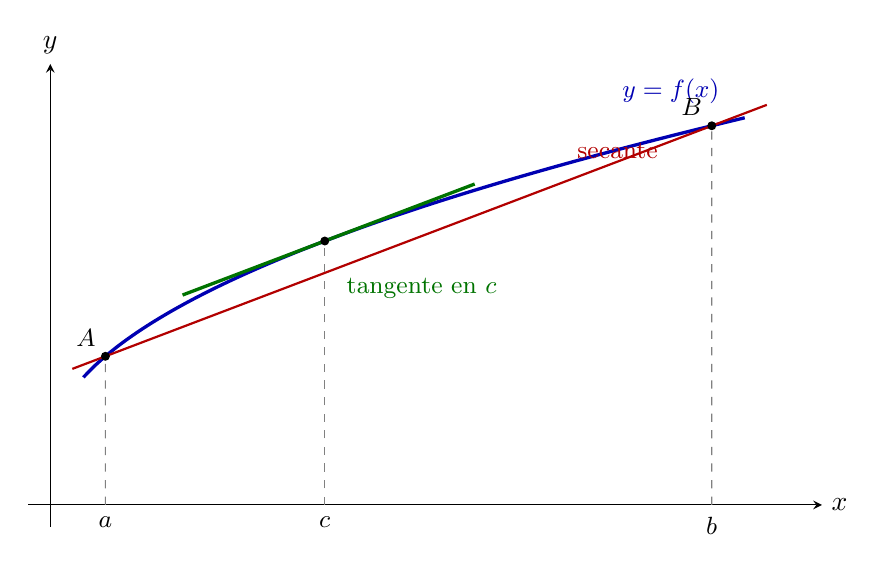
\begin{tikzpicture}[scale=1.4,>=stealth]
  \draw[->,thin] (-0.2,0)--(7,0) node[right]{$x$};
  \draw[->,thin] (0,-0.2)--(0,4) node[above]{$y$};
  % curva f(x)=1.2 sqrt(x)+0.5
  \draw[very thick,blue!70!black,domain=0.3:6.3,samples=60,smooth]
    plot(\x,{1.2*sqrt(\x)+0.5});
  \node[blue!70!black,anchor=west,font=\small] at (5.1,3.75) {$y=f(x)$};
  % puntos A, B
  \coordinate (A) at (0.5,1.348);
  \coordinate (B) at (6,3.439);
  % secante (pendiente 0.38)
  \draw[red!70!black,thick] (0.2,1.234)--(6.5,3.629);
  % tangente en c=2.49 (misma pendiente)
  \draw[very thick,green!45!black] (1.2,1.904)--(3.85,2.911);
  % verticales
  \draw[dashed,gray] (2.49,0)--(2.49,2.394);
  \draw[dashed,gray] (0.5,0)--(A);
  \draw[dashed,gray] (6,0)--(B);
  % marcas
  \filldraw (A) circle(1pt) node[above left,font=\small]{$A$};
  \filldraw (B) circle(1pt) node[above left,font=\small]{$B$};
  \filldraw (2.49,2.394) circle(1pt);
  \node[below,font=\small] at (0.5,-0.02) {$a$};
  \node[below,font=\small] at (2.49,-0.02) {$c$};
  \node[below,font=\small] at (6,-0.02) {$b$};
  % etiquetas de rectas
  \node[red!70!black,font=\small,anchor=south east] at (5.6,3.05) {secante};
  \node[green!45!black,font=\small,anchor=north west] at (2.6,2.15) {tangente en $c$};
\end{tikzpicture}
\caption{Teorema del Valor Medio: existe $c\in(a,b)$ donde la recta tangente
  (verde) es paralela a la secante (roja) que une $A=(a,f(a))$ con
  $B=(b,f(b))$; en ese punto $f'(c)=\dfrac{f(b)-f(a)}{b-a}$.}
\label{fig:tvm_secante_tangente}
\end{figure}

\begin{example}[Demostración del TVM a partir de Rolle]
Demostrar el Teorema del Valor Medio a partir del Lema de Rolle.
\begin{myproof}
\textbf{Paso 1. Definir la función auxiliar.}

La idea es «aplanar» la secante para reducir el problema al caso de
Rolle. Se define:
\[
h(x) = f(x) - f(a) - \frac{f(b)-f(a)}{b-a}(x-a).
\]
Geométricamente, $h(x)$ mide la distancia vertical entre la curva $f$
y la recta secante que une $(a,f(a))$ con $(b,f(b))$.

\textbf{Paso 2. Verificar las hipótesis del Lema de Rolle para $h$.}

\begin{itemize}
    \item $h$ es continua en $[a,b]$ y derivable en $(a,b)$, pues $f$
    lo es y la función lineal restada también.
    \item $h(a) = f(a)-f(a)-0 = 0$.
    \item $h(b) = f(b)-f(a)-\dfrac{f(b)-f(a)}{b-a}(b-a) = 0$.
\end{itemize}

Las tres hipótesis del Lema de Rolle se satisfacen.

\textbf{Paso 3. Aplicar Rolle y concluir.}

Como $h(a)=h(b)=0$, el Lema de Rolle garantiza $c\in(a,b)$ con
$h'(c)=0$. Calculando $h'$:
\[
h'(x) = f'(x) - \frac{f(b)-f(a)}{b-a},
\]
de modo que $h'(c)=0$ equivale exactamente a:
\[
\boxed{f'(c) = \frac{f(b)-f(a)}{b-a}.}
\]
\end{myproof}
\end{example}

Una consecuencia inmediata del TVM es el siguiente corolario, que
constituye el fundamento teórico de la integración indefinida.

\begin{coro}
Si $F'(x)=G'(x)$ para todo $x\in(a,b)$, entonces $F(x)=G(x)+C$
para alguna constante $C$.
\end{coro}

\begin{rem}
Este corolario justifica el ``$+C$'' que aparece en toda antiderivada:
dos funciones que tienen la misma derivada en un intervalo solo pueden
diferir en una constante aditiva. Sin el TVM, esta afirmación, que
parece obvia, carecería de demostración rigurosa.
\end{rem}

\begin{example}[Verificación del TVM para $f(x)=x^3-x$]
Verificar el Teorema del Valor Medio para $f(x)=x^3-x$ en $[0,2]$
y encontrar el valor $c$ garantizado por el teorema.
\begin{myproof}
Como $f$ es un polinomio, es continua en $[0,2]$ y derivable en
$(0,2)$, por lo que el TVM es aplicable.

\textbf{Paso 1. Calcular la pendiente de la recta secante.} \(
f(0) = 0, \qquad f(2) = 8-2 = 6.
\)
La pendiente de la secante que une los extremos del intervalo es:
\[
m = \frac{f(2)-f(0)}{2-0} = \frac{6-0}{2} = 3.
\]

\textbf{Paso 2. Igualar la derivada a dicha pendiente.} \(
f'(x) = 3x^2 - 1.
\) El TVM garantiza que existe $c\in(0,2)$ tal que $f'(c)=3$:
\[
3c^2 - 1 = 3 \implies c^2 = \frac{4}{3} \implies c = \frac{2}{\sqrt{3}}
= \frac{2\sqrt{3}}{3} \approx 1.155.
\]
La raíz negativa $c=-\dfrac{2}{\sqrt{3}}$ queda fuera de $(0,2)$ y
se descarta.

\textbf{Paso 3. Verificar.}

El valor $c=\dfrac{2\sqrt{3}}{3}\approx 1.155$ pertenece efectivamente
a $(0,2)$, lo que confirma la conclusión del TVM: en ese punto la
tangente a la curva es paralela a la recta secante de pendiente $3$.
\[
\boxed{c = \frac{2\sqrt{3}}{3} \approx 1.155.}
\]
\end{myproof}
\end{example}

%%==========================================================
\section{Regla de L'Hôpital}
%%==========================================================

Al calcular límites, es frecuente encontrar expresiones donde numerador
y denominador tienden simultáneamente a cero o a infinito. En estos
casos, la forma del cociente no permite determinar directamente el valor
del límite, pues se obtienen expresiones sin significado algebraico
definido como $\frac{0}{0}$ o $\frac{\infty}{\infty}$: se habla
entonces de \textbf{formas indeterminadas}. La Regla de L'Hôpital
ofrece una herramienta sistemática para resolver esta clase de límites
recurriendo a las derivadas del numerador y del denominador. Su
potencia radica en que convierte un problema de límites en un nuevo
problema de límites (generalmente más sencillo)
 sin alterar el valor
buscado. Sin embargo, debe aplicarse con precisión: solo es válida
bajo condiciones específicas, y su uso incorrecto conduce a resultados
erróneos.

\begin{theorem}[Regla de L'Hôpital]
Supóngase que $\lim_{x\to a}f(x)=0$ y $\lim_{x\to a}g(x)=0$ tiene forma
$\frac{0}{0}$, o que ambos tienden a $\pm\infty$ tiene forma
$\frac{\infty}{\infty}$. Si $f$ y $g$ son derivables cerca de $a$,
$g'(x)\neq 0$ allí, y el límite $\lim_{x\to a}\frac{f'(x)}{g'(x)}$
existe (o es $\pm\infty$), entonces
\[
\lim_{x\to a}\frac{f(x)}{g(x)} = \lim_{x\to a}\frac{f'(x)}{g'(x)}.
\]
El resultado también vale para $a=\pm\infty$ y para límites laterales.
\end{theorem}

\begin{rem}
La regla exige derivar \textbf{numerador y denominador por separado},
no aplicar la regla del cociente. Dos errores frecuentes merecen
atención especial: el primero es aplicarla cuando el límite \emph{no} es una
forma indeterminada, lo que produce resultados incorrectos; y el segundo aplicarla
repetidamente sin verificar que el nuevo cociente siga siendo
indeterminado. Si tras una aplicación el límite permanece indeterminado,
la regla puede reiterarse; si el cociente de derivadas oscila sin
converger, conviene buscar un método alternativo.
\end{rem}

Además de $\frac{0}{0}$ y $\frac{\infty}{\infty}$, existen otras formas
indeterminadas que no son cocientes directos. La tabla siguiente muestra
cómo reducirlas a una de las dos formas en que L'Hôpital es aplicable.

\begin{center}
\renewcommand{\arraystretch}{1.6}
\begin{tabular}{l l l}
\toprule
\textbf{Forma} & \textbf{Transformación} & \textbf{Reduce a} \\
\midrule
$0\cdot\infty$ &
  $f\cdot g = \dfrac{f}{1/g}$ \ o \ $\dfrac{g}{1/f}$ &
  $0/0$ \ o \ $\infty/\infty$ \\
$\infty-\infty$ &
  denominador común o racionalización &
  $0/0$ \\
$0^0,\;1^\infty,\;\infty^0$ &
  $y=f^g \Rightarrow \ln y = g\ln f$; hallar $\lim\ln y = L$ &
  $0/0$ \ o \ $\infty/\infty$; resultado: $e^L$ \\
\bottomrule
\end{tabular}
\end{center}

Los cuatro ejemplos que siguen ilustran cada tipo de forma indeterminada.

% ============================================================
\begin{example}[L'Hôpital: forma $0/0$ con doble aplicación]
Calcular $\displaystyle\lim_{x\to 0}\frac{e^x-1-x}{x^2}$.
\begin{myproof}
\textbf{Paso 1. Identificar la forma indeterminada.}

Al sustituir $x=0$ se obtiene $\dfrac{e^0-1-0}{0^2}=\dfrac{0}{0}$:
forma indeterminada; L'Hôpital es aplicable.

\textbf{Paso 2. Primera aplicación de L'Hôpital.}

Se derivan numerador y denominador por separado:
\[
\lim_{x\to 0}\frac{e^x-1-x}{x^2}
\overset{\text{L'H}}{=}
\lim_{x\to 0}\frac{e^x-1}{2x}.
\]
Al sustituir $x=0$: $\dfrac{0}{0}$. La forma sigue siendo indeterminada;
se aplica la regla una segunda vez.

\textbf{Paso 3. Segunda aplicación y conclusión.}

\[
\lim_{x\to 0}\frac{e^x-1}{2x}
\overset{\text{L'H}}{=}
\lim_{x\to 0}\frac{e^x}{2}
= \frac{e^0}{2} = \frac{1}{2}.
\]
\[
\boxed{\lim_{x\to 0}\frac{e^x-1-x}{x^2} = \frac{1}{2}.}
\]
\end{myproof}
\end{example}

% ============================================================
\begin{example}[L'Hôpital: forma $\infty\cdot 0$]
Calcular $\displaystyle\lim_{x\to\infty}x\,e^{-x}$.
\begin{myproof}
\textbf{Paso 1. Identificar la forma e transformar en cociente.}

Cuando $x\to\infty$, el factor $x\to\infty$ y el factor $e^{-x}\to 0$:
forma indeterminada $\infty\cdot 0$. L'Hôpital no se aplica a productos;
se reescribe poniendo $e^{-x}$ en el denominador:
\[
\lim_{x\to\infty} x\,e^{-x}
= \lim_{x\to\infty}\frac{x}{e^{x}}.
\]
Ahora la forma es $\dfrac{\infty}{\infty}$, sobre la que L'Hôpital sí actúa.

\textbf{Paso 2. Aplicar L'Hôpital y concluir.}

\[
\lim_{x\to\infty}\frac{x}{e^{x}}
\overset{\text{L'H}}{=}
\lim_{x\to\infty}\frac{1}{e^{x}} = 0.
\]
El exponencial domina al polinomio:
\[
\boxed{\lim_{x\to\infty}x\,e^{-x} = 0.}
\]
\end{myproof}
\end{example}

% ============================================================
\begin{example}[L'Hôpital: forma $0^0$]
Calcular $\displaystyle\lim_{x\to 0^+}x^x$.
\begin{myproof}
\textbf{Paso 1. Identificar la forma e introducir la estrategia logarítmica.}

Cuando $x\to 0^+$, la base tiende a $0$ y el exponente también: forma
indeterminada $0^0$. Sea $y=x^x$; tomando logaritmo natural:
\[
\ln y = x\ln x.
\]

\textbf{Paso 2. Transformar en cociente y aplicar L'Hôpital.}

Cuando $x\to 0^+$, $x\ln x$ es $0\cdot(-\infty)$. Se reescribe como cociente:
\[
\lim_{x\to 0^+} x\ln x
= \lim_{x\to 0^+}\frac{\ln x}{1/x}
\overset{\text{L'H}}{=}
\lim_{x\to 0^+}\frac{1/x}{-1/x^2}
= \lim_{x\to 0^+}(-x) = 0.
\]
Luego $\lim_{x\to 0^+}\ln y = 0$.

\textbf{Paso 3. Recuperar el límite original.}

Como la función exponencial es continua, se pasa el límite al exponente:
\[
\lim_{x\to 0^+} y = e^{\,\lim\ln y} = e^0 = 1.
\]
\[
\boxed{\lim_{x\to 0^+}x^x = 1.}
\]
\end{myproof}
\end{example}

% ============================================================
\begin{example}[L'Hôpital: forma $1^\infty$]
Calcular $\displaystyle\lim_{x\to\infty}\!\left(1+\frac{a}{x}\right)^{\!x}$.
\begin{myproof}
\textbf{Paso 1. Identificar la forma e introducir la estrategia logarítmica.}

Cuando $x\to\infty$, la base tiende a $1$ y el exponente a $\infty$:
forma indeterminada $1^\infty$. Sea $y=\!\left(1+\dfrac{a}{x}\right)^{\!x}$;
tomando logaritmo natural:
\[
\ln y = x\ln\!\left(1+\frac{a}{x}\right).
\]

\textbf{Paso 2. Transformar en cociente y aplicar L'Hôpital.}

Cuando $x\to\infty$, esto es $\infty\cdot 0$. Se reescribe como cociente:
\[
\lim_{x\to\infty} x\ln\!\left(1+\frac{a}{x}\right)
= \lim_{x\to\infty}\frac{\ln(1+a/x)}{1/x}.
\]
La forma es $\dfrac{0}{0}$. Derivando numerador y denominador respecto a $x$:
\[
\overset{\text{L'H}}{=}
\lim_{x\to\infty}
\frac{\dfrac{1}{1+a/x}\cdot\dfrac{-a}{x^2}}{-\,\dfrac{1}{x^2}}
= \lim_{x\to\infty}\frac{a}{1+a/x}
= a.
\]
Luego $\lim_{x\to\infty}\ln y = a$.

\textbf{Paso 3. Recuperar el límite original.}

Por continuidad del exponencial:
\[
\boxed{\lim_{x\to\infty}\!\left(1+\frac{a}{x}\right)^{\!x} = e^a.}
\]
En particular, para $a=1$ se recupera el límite notable
$\lim_{x\to\infty}\!\left(1+\dfrac{1}{x}\right)^{\!x}=e$.
\end{myproof}
\end{example}

%%==========================================================
\section{Métodos Numéricos para la Localización de Raíces}
%%==========================================================

Las herramientas del cálculo diferencial permiten analizar y graficar
funciones con precisión, pero no siempre garantizan expresiones cerradas
para sus raíces. Ecuaciones como $e^x = 3x$ o $\cos x = x$ no admiten
solución algebraica exacta, y sin embargo sus raíces tienen plena
existencia y significado. En estos casos se recurre a los
\textbf{métodos numéricos}: algoritmos iterativos que construyen
sucesiones de aproximaciones cada vez más próximas a la raíz buscada.
En esta sección se estudian tres métodos clásicos, los métodos de bisección,
Newton-Raphson y punto fijo, cada uno con distintos requisitos,
velocidad de convergencia y grado de robustez. La tabla al final de la
sección permite compararlos de un vistazo.

%%----------------------------------------------------------
\subsection{Bisección}
%%----------------------------------------------------------

El método de bisección es una aplicación directa del Teorema del Valor
Intermedio (Bolzano): si $f$ es continua en $[a,b]$ y $f(a)\cdot
f(b)<0$, la función cambia de signo en el intervalo y, por tanto,
tiene al menos una raíz en su interior. El método explota esta
garantía de forma sistemática: en cada paso se evalúa el punto medio
$m=\dfrac{a+b}{2}$ y se determina en cuál de los dos subintervalos
$[a,m]$ o $[m,b]$ persiste el cambio de signo; ese subintervalo se
convierte en el nuevo intervalo de búsqueda y el proceso se repite.
Tras $n$ iteraciones, la raíz está acotada con un error menor que
\[
\varepsilon_n < \frac{b-a}{2^n},
\]
lo que permite estimar de antemano cuántas iteraciones son necesarias
para alcanzar una precisión dada.

\begin{rem}
La bisección es el método más \textbf{robusto}: converge siempre que
se cumplan las hipótesis de continuidad y cambio de signo, sin importar
la forma de $f$. Su desventaja es la velocidad: la convergencia es
\textbf{lineal}, es decir, el número de cifras decimales correctas
crece a razón de una cifra cada $\log_2 10 \approx 3.32$ iteraciones.
Para obtener $k$ cifras adicionales de precisión se requieren
aproximadamente $3.32\,k$ iteraciones.
\end{rem}

%%----------------------------------------------------------
\subsection{Método de Newton-Raphson}
%%----------------------------------------------------------

El método de Newton-Raphson parte de una idea geométrica: si se conoce
una aproximación $x_n$ a la raíz, la recta tangente a la curva en el
punto $(x_n, f(x_n))$ suele cruzar el eje $x$ en un punto $x_{n+1}$
más próximo a la raíz verdadera. Repitiendo este proceso se construye
la sucesión:
\[
x_{n+1} = x_n - \frac{f(x_n)}{f'(x_n)}.
\]
\begin{example}[Derivación geométrica de la fórmula de Newton-Raphson]
Construir geométricamente la fórmula iterativa del método de Newton-Raphson.
\begin{myproof}
\textbf{Paso 1. Escribir la ecuación de la recta tangente en $(x_n,f(x_n))$.}

La recta tangente a $f$ en el punto $(x_n,f(x_n))$ tiene ecuación:
\[
y - f(x_n) = f'(x_n)(x - x_n).
\]

\textbf{Paso 2. Hallar la intersección con el eje $x$ y definir $x_{n+1}$.}

Se iguala $y=0$ para encontrar la intersección:
\[
x = x_n - \frac{f(x_n)}{f'(x_n)} =: x_{n+1}.
\]
\[
\boxed{x_{n+1} = x_n - \frac{f(x_n)}{f'(x_n)}.}
\]
\end{myproof}
\end{example}
La convergencia de Newton-Raphson es \textbf{cuadrática}: el número de
cifras decimales correctas se \emph{duplica} en cada iteración cuando
la aproximación es suficientemente cercana a la raíz. Esta velocidad
lo convierte en el método preferido en la práctica. Sin embargo,
presenta limitaciones importantes: falla si $f'(x_n)=0$ en algún paso
(división por cero), puede diverger si la aproximación inicial $x_0$
está lejos de la raíz, y es sensible a oscilaciones de $f$ que desvíen
las iteraciones. La elección de un buen punto de partida, guiada por
el análisis previo de la función, es parte esencial de su uso correcto.

\begin{example}[Newton-Raphson: aproximación de $\sqrt{2}$]
Aproximar $\sqrt{2}$ resolviendo $f(x)=x^2-2=0$ con Newton-Raphson
y valor inicial $x_0=1$.
\begin{myproof}
\textbf{Paso 1. Plantear la fórmula iterativa.}

Con $f(x)=x^2-2$ y $f'(x)=2x$, la fórmula general se simplifica a la
\emph{media aritmética de $x_n$ y $2/x_n$}:
\[
x_{n+1} = x_n - \frac{x_n^2-2}{2x_n} = \frac{x_n + 2/x_n}{2}.
\]

\textbf{Paso 2. Aplicar la iteración y tabular los resultados.}

Partiendo de $x_0=1$:

\begin{center}
\begin{tabular}{c l}
\toprule
$n$ & \multicolumn{1}{c}{$x_n$} \\
\midrule
$0$ & $1$ \\
$1$ & $1.5$ \\
$2$ & $1.41\overline{6}$ \\
$3$ & $1.41421356\ldots$ \\
\bottomrule
\end{tabular}
\end{center}

\textbf{Paso 3. Interpretar la convergencia.}

Con tres iteraciones se obtienen ocho cifras decimales correctas,
ilustrando la convergencia cuadrática del método.
\[
\boxed{\sqrt{2} \approx x_3 = 1.41421356\ldots}
\]
\end{myproof}
\end{example}

%%----------------------------------------------------------
\subsection{Método de Punto Fijo}
%%----------------------------------------------------------

El método de punto fijo aborda la ecuación $f(x)=0$ desde una
perspectiva distinta: se reescribe algebraicamente en la forma
$x=g(x)$ y se itera la sucesión $x_{n+1}=g(x_n)$. Un
\textbf{punto fijo} de $g$ es un valor $x^*$ tal que $g(x^*)=x^*$; si
la reescritura es correcta, todo punto fijo de $g$ es raíz de $f$.
La convergencia de la sucesión depende de qué tan fuertemente $g$
«contrae» el espacio en torno a $x^*$.

\begin{theorem}[Convergencia del punto fijo]
Si $|g'(x)|<1$ para todo $x$ en un intervalo que contiene a la raíz,
las iteraciones $x_{n+1}=g(x_n)$ convergen a ella desde cualquier
punto inicial en ese intervalo.
\end{theorem}

\begin{rem}
La condición $|g'(x)|<1$ se denomina \textbf{condición de
contracción}: garantiza que $g$ acerca entre sí los puntos sucesivos
en cada iteración. Si $|g'(x)|>1$, las iteraciones se alejan de la
raíz. La reescritura $x=g(x)$ no es única: una misma ecuación puede
admitir versiones convergentes y divergentes, por lo que elegir la
adecuada es parte esencial del método. En la práctica, Newton-Raphson
es un caso particular de punto fijo con $g(x)=x-\dfrac{f(x)}{f'(x)}$,
cuya condición de contracción se satisface automáticamente cerca de
raíces simples.
\end{rem}

Finalmente se realiza una comparación de los tres métodos
\begin{center}
\renewcommand{\arraystretch}{1.6}
\begin{tabular}{l l l l}
\toprule
\textbf{Método} & \textbf{Convergencia} & \textbf{Robustez}
& \textbf{Requisitos} \\
\midrule
Bisección      & Lineal      & Alta  &
  $f$ continua y cambio de signo en $[a,b]$ \\
Newton-Raphson & Cuadrática  & Media &
  $f$ derivable y buena aproximación $x_0$ \\
Punto fijo     & Lineal/variable & Baja  &
  $|g'|<1$ en un entorno de la raíz \\
\bottomrule
\end{tabular}
\end{center}

%%==========================================================
\section{Diferenciales y Aproximaciones Lineales}
%%==========================================================

Cuando $f'(a)$ existe, la recta tangente en $(a,f(a))$ es la mejor
aproximación lineal de $f$ cerca de $a$. Esta idea se formaliza
mediante el concepto de \textbf{diferencial} y la
\textbf{linealización}, herramientas que permiten estimar cambios
en los valores de $f$ sin calcular raíces ni integrales.

\begin{definition}
Sea $f$ derivable en $x$. El \textbf{diferencial de $f$} es la expresión
\[
df = f'(x)\,dx,
\]
donde $dx$ es un incremento arbitrario en $x$. El diferencial $df$
aproxima el cambio real $\Delta f = f(x+dx)-f(x)$ cuando $|dx|$
es pequeño.
\end{definition}

\begin{rem}
La diferencia entre el cambio real $\Delta y$ y el diferencial $dy$
es del orden de $(dx)^2$ para funciones suaves:
$\Delta y = dy + \mathcal{O}\!\left((dx)^2\right)$.
Cuando $|dx|\ll 1$, el error relativo $(\Delta y - dy)/\Delta y$
también es pequeño, por lo que $dy$ es una aproximación práctica útil.
\end{rem}

\begin{theorem}[Aproximación lineal o linealización]
Si $f$ es derivable en $a$, entonces para $x$ cerca de $a$:
\[
f(x) \approx L(x) = f(a) + f'(a)(x - a).
\]
$L(x)$ se denomina la \textbf{linealización de $f$ en $a$}; su gráfica
es la recta tangente a $f$ en el punto $(a,f(a))$.
\end{theorem}

\begin{pasos}
Para estimar $f(b)$ cuando $b$ está cerca de un punto $a$ conveniente:
\begin{enumerate}
    \item Elegir $a$ cercano a $b$ donde $f(a)$ sea exactamente
    calculable.
    \item Calcular $f'(a)$.
    \item Aplicar: $f(b) \approx f(a) + f'(a)(b-a)$.
\end{enumerate}
\end{pasos}

\begin{example}[Aproximación lineal de $\sqrt{4.02}$]
Usar la aproximación lineal para estimar $\sqrt{4.02}$.
\begin{myproof}
\textbf{Paso 1. Elegir el punto base.}

Se toma $f(x)=\sqrt{x}$ y $a=4$, pues $f(4)=\sqrt{4}=2$ es exacto.

\textbf{Paso 2. Calcular $f'(a)$.}

\[
f'(x) = \frac{1}{2\sqrt{x}} \implies f'(4) = \frac{1}{4}.
\]

\textbf{Paso 3. Aplicar la aproximación lineal.}

Con $b=4.02$ y $b-a=0.02$:
\[
\sqrt{4.02} \approx f(4) + f'(4)(4.02-4)
= 2 + \frac{1}{4}(0.02) = \boxed{2.005}.
\]
El valor exacto es $\sqrt{4.02}\approx 2.00499\ldots$; el error
absoluto es menor que $0.00001$.
\end{myproof}
\end{example}

\begin{example}[Aproximación lineal de $\sen 31^\circ$]
Usar la aproximación lineal para estimar $\sen 31^\circ$.
\begin{myproof}
\textbf{Paso 1. Elegir el punto base.}

Se trabaja en radianes: $31^\circ = \dfrac{31\pi}{180}$ rad, cercano
a $a=\dfrac{\pi}{6}$ ($=30^\circ$), para el que $\sen\dfrac{\pi}{6}=\dfrac{1}{2}$
es exacto.

\textbf{Paso 2. Calcular $f'(a)$.}

Con $f(x)=\sen x$:
\[
f'(x)=\cos x \implies f'\!\left(\frac{\pi}{6}\right)=\cos\frac{\pi}{6}
=\frac{\sqrt{3}}{2}.
\]

\textbf{Paso 3. Aplicar la aproximación lineal.}

El incremento es $\Delta x=\dfrac{\pi}{180}$ rad ($=1^\circ$):
\[
\sen 31^\circ \approx \frac{1}{2}+\frac{\sqrt{3}}{2}\cdot\frac{\pi}{180}
\approx 0.5000 + 0.0151 = \boxed{0.5151}.
\]
El valor exacto es $\sen 31^\circ\approx 0.5150\ldots$; error menor que $0.0001$.
\end{myproof}
\end{example}

%%==========================================================
\section{Problemas propuestos}
%%==========================================================
\begin{prob}
Determine el valor de verdad de las siguientes afirmaciones.
Justifique su respuesta.
\begin{enumerate}
    \item La función $f(x)=\dfrac{x+1}{x-1}$ en el intervalo
    $[-2,-1]$ satisface las hipótesis del Teorema del Valor Medio.

    \item La recta tangente a $f(x)=5-x^2+e^{2x-2}$ es horizontal
    en el punto $(1,5)$.

    \item Si $f$ es derivable y $f(-1)=f(1)$, entonces existe
    $c\in(-1,1)$ tal que $f'(c)=0$.

    \item Si $f$ es creciente y positiva en $I$, entonces
    $g(x)=\dfrac{1}{f(x)}$ es positiva y decreciente en $I$.

    \item El valor de
    $\displaystyle\lim_{x\to\infty}\frac{\sqrt{1+x^2}}{x+1}$ es $1$.

    \item El dominio de $f(x)=\sqrt{2x+5}+\ln(6-8x)$ es
    $\left[-\dfrac{5}{2},\,\dfrac{3}{4}\right)$.
\end{enumerate}
\end{prob}


\subsection{Razones de cambio relacionadas}

% Básico
\begin{prob}
El radio de un círculo crece a razón de $3$ cm/s. ¿A qué tasa crece
el área cuando el radio mide $10$ cm?
\end{prob}

\begin{prob}
Dos autos parten desde una intersección: uno hacia el norte a $60$
km/h y otro hacia el este a $80$ km/h. ¿A qué velocidad se separan
$2$ horas después?
\end{prob}

\begin{prob}
Un globo esférico pierde aire a razón de $2$ cm$^3$/min. ¿A qué tasa
decrece el radio cuando $r=5$ cm?
\end{prob}

\begin{prob}
Se deja caer una pelota desde una altura de $100$ pies. Un segundo después, se deja caer otra pelota desde una altura de $75$ pies. ¿Cuál de ellas llega primero al suelo?
\end{prob}

% Intermedio
\begin{prob}
Una cámara está situada $500$ m de la base de un cohete en lanzamiento
vertical. ¿A qué velocidad angular debe girar la cámara para seguir
al cohete cuando este ha alcanzado $500$ m de altura y sube a $300$ m/s?
\end{prob}

\begin{prob}
Un depósito tiene forma de tronco de cono, su radio inferior mide $2$ m mientras que el radio superior mide $4$ m y su altura mide $6$ m. Este depósito se está llenando con agua a $3$ m$^3$/min.
¿A qué velocidad sube el nivel cuando $h=3$ m?
\end{prob}

\begin{prob}
Una embarcación parte al mediodía hacia el Norte a $30$ km/h. Una hora
después, una segunda embarcación parte del mismo lugar hacia el Este a
$40$ km/h. ¿Con qué rapidez se separan las dos embarcaciones a la
$1{:}30$ pm?
\end{prob}

\begin{prob}
Un vaso de papel tiene forma cónica de altura $12$ cm y radio $4$ cm
en la parte superior. Si se vierte agua a razón de $3$ cm$^3$/s,
¿qué tan rápido sube el nivel cuando la profundidad es de $6$ cm?
\end{prob}

\begin{prob}
De un tanque hemisférico de radio $10$ m entra agua a razón de
$1$ m$^3$/min y sale por un orificio inferior a razón de
$\dfrac{1}{5}$ m$^3$/min. ¿A qué razón cambia la altura $h$ del agua
cuando la profundidad es de $5$ m?
\end{prob}

\begin{prob}
Un cuadrado está inscrito en un círculo de radio $r$. ¿A qué razón
cambia el área del cuadrado cuando el radio del círculo crece a razón
de $4$ pulg/min? Vea la figura~\ref{fig:cuadrado_inscrito}.
\begin{figure}[H]
\centering
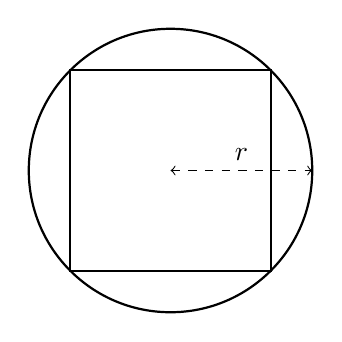
\begin{tikzpicture}[scale=0.9]
  \draw[thick] (0,0) circle (2);
  \draw[thick] (-1.414,-1.414) rectangle (1.414,1.414);
  \draw[<->,dashed] (0,0)--(2,0) node[midway,above]{$r$};
\end{tikzpicture}
\caption{Cuadrado inscrito en una circunferencia de radio $r$: la diagonal
  del cuadrado es el diámetro $2r$, de modo que su lado es $r\sqrt2$.}
\label{fig:cuadrado_inscrito}
\end{figure}
\end{prob}

\begin{prob}
Un niño viaja en bicicleta a una velocidad constante de $15$ pies/s a lo largo
de un camino recto (Eje $x$). Un globo aerostático asciende verticalmente a
$5$ pies/s, manteniendo siempre una distancia lateral fija de $45$ pies
respecto al camino (Eje $y$). Si en el tiempo $t=0$ el niño se encuentra en
el punto del camino más cercano al globo, ¿con qué rapidez incrementa la
distancia entre ellos $3$ segundos después?

\begin{figure}[H]
\centering
\tdplotsetmaincoords{70}{110}
\begin{tikzpicture}[tdplot_main_coords, scale=0.08, >=stealth]

    % --- Ejes de Coordenadas ---
    \draw[->, thick] (0,0,0) -- (80,0,0) node[anchor=north east]{$x$ (Camino)};
    \draw[->, thick] (0,0,0) -- (0,70,0) node[anchor=west]{$y$ (Separación)};
    \draw[->, thick] (0,0,0) -- (0,0,60) node[anchor=south]{$z$ (Altura)};

    % --- Puntos Clave ---
    \coordinate (O)    at (0,0,0);
    \coordinate (N)    at (45,0,0);   % Niño a t=3s: x = 15*3 = 45
    \coordinate (P)    at (0,45,0);   % Proyección del globo en el suelo
    \coordinate (G)    at (0,45,15);  % Globo a t=3s: y=45, z=5*3=15
    \coordinate (Base) at (45,45,0);  % Esquina del triángulo base

    % --- Líneas de construcción ---
    \draw[dashed, blue!60] (O)    -- (P)    node[midway, sloped, above]{45 ft};
    \draw[dashed, blue!60] (P)    -- (Base);
    \draw[dashed, blue!60] (N)    -- (Base) node[midway, sloped, below]{45 ft};
    \draw[dashed, red!60]  (Base) -- (G)    node[midway, right]{$z=15$ ft};

    % --- Vector de distancia L ---
    \draw[ultra thick, red, ->] (N) -- (G)
        node[midway, above, sloped]{$L(t)$};

    % --- El Niño ---
    \filldraw[black] (N) circle (1.5pt);
    \node[anchor=north] at (45,0,-2) {Niño ($x=45$)};

    % --- El Globo ---
    \shade[ball color=blue!40, opacity=0.8] (G) circle (4pt);
    \draw (G) -- (0,45,10);
    \node[anchor=south] at (0,45,20) {Globo ($z=15$)};

    % --- Ángulos rectos ---
    \draw[thin] (0,2,0)  -- (2,2,0)   -- (2,0,0);   % en plano x-y
    \draw[thin] (45,45,2)-- (45,43,2) -- (45,43,0);  % en elevación

\end{tikzpicture}
\caption{Niño en bicicleta sobre el eje $x$ y globo que asciende
  manteniendo una separación lateral fija de $45$ ft; $L(t)$ es la distancia
  entre ambos a los $3$ s.}
\label{fig:nino_globo}
\end{figure}
\end{prob}

% Desafiante
\begin{prob}
Un tanque lleno de agua tiene forma de cilindro recto de bases con
diámetro $2$ m y altura $6$ m. Dentro hay un sólido cónico invertido
cuya base coincide con la tapa superior del cilindro. Si el agua sale
a razón de $\dfrac{1}{3}$ m$^3$/hr, ¿con qué rapidez desciende el
nivel del agua cuando la profundidad es de $3$ m?
\end{prob}

\begin{prob}
Un recipiente cónico invertido tiene altura $16$ cm y radio $5$ cm en
la parte superior. Un líquido escurre por las paredes a una tasa
proporcional al área lateral en contacto con el líquido. Si se vierte
líquido a razón de $2$ cm$^3$/min, el nivel desciende a $0.3$ cm/min
cuando la altura del líquido es $10$ cm. ¿Con qué rapidez debe
verterse líquido para mantener una altura constante de $10$ cm? Recuerde que el área lateral de un cono es \(A=\pi r\ell.\)
\end{prob}

\begin{prob}
Un cono de radio $r$ cm y altura $h$ cm es introducido punta abajo a
$2$ cm/s dentro de un cilindro de radio $R$ cm que contiene agua a
altura $h_2$. ¿Qué tan rápido sube el nivel del agua en el instante
en que el cono queda totalmente sumergido?
\end{prob}

% Requiere en el preámbulo: \usepackage{amsmath,amssymb,float,tikz}
% \usetikzlibrary{calc,angles,quotes}

\begin{prob}
  El dispositivo mostrado en la figura consta de dos ruedas dentadas, $A$ y $B$, conectadas por una cadena que no desliza. Un brazo extendible une un punto fijo $P$ con un punto $T$ situado sobre el borde de la rueda $B$. El segmento $PO$ mide $4$ dm, y los radios de las ruedas $A$ y $B$ son $1$ dm y $2$ dm, respectivamente. Los segmentos $AO$ y $OP$ son perpendiculares. La rueda $A$ gira a razón de una vuelta por segundo en sentido antihorario. Si inicialmente el punto $T$ se encuentra sobre el segmento $OP$, ¿con qué rapidez cambia la longitud $x = PT$ cuando el ángulo $\theta = \angle POT$ es de $60^\circ$?

  \begin{figure}[H]
    \centering
    \begin{tikzpicture}[scale=0.85, every node/.style={font=\small}, >=stealth]
      % Parámetros geométricos
      \def\thetaVal{60}
      \def\chainAngle{7.18} % asin((r_B-r_A)/AO) = asin(1/8) en grados

      % Coordenadas principales
      \coordinate (A) at (0,0);
      \coordinate (O) at (8,0);
      \coordinate (P) at (8,4);
      \coordinate (T) at ($(O) + (90+\thetaVal:2)$);

      % Puntos de tangencia para la cadena externa
      \coordinate (At) at ($(A) + (90+\chainAngle:1)$);
      \coordinate (Ab) at ($(A) + (270-\chainAngle:1)$);
      \coordinate (Ot) at ($(O) + (90+\chainAngle:2)$);
      \coordinate (Ob) at ($(O) + (270-\chainAngle:2)$);

      % Ruedas y cadena
      \draw[thick] (A) circle[radius=1];
      \draw[thick] (O) circle[radius=2];
      \draw[thick] (At) -- (Ot);
      \draw[thick] (Ab) -- (Ob);
       % Arcos de contacto de la cadena (CORREGIDO)
      \draw[thick] (Ot) arc[start angle=90+\chainAngle, end angle=270-\chainAngle, radius=2];
      \draw[thick] (Ab) arc[start angle=270-\chainAngle, end angle=90+\chainAngle, radius=1];

      % Segmentos geométricos
      \draw[thick] (A) -- (O) node[midway, below] {$h$};
      \draw[thick] (O) -- (P) node[midway, above] {$4$ dm};
      \draw[thick] (O) -- (T);
      \draw[thick] (P) -- (T) node[midway, above left] {$x$};

      % Ángulo theta
      \pic[draw, fill=gray!20, "$\theta=60^\circ$", angle eccentricity=1.4, angle radius=12mm] {angle = P--O--T};

      % Indicadores de rotación (antihorario)
      \draw[->, thick, blue!70!black] ($(A) + (30:1.3)$) arc[start angle=30, end angle=150, radius=1.3];
      \draw[->, thick, blue!70!black] ($(O) + (30:2.3)$) arc[start angle=30, end angle=150, radius=2.3];
      \draw[->, thick, blue!70!black] ($(At)!0.5!(Ot) + (0,0.3)$) -- ++(-0.8,0) node[left, font=\footnotesize] {cadena};

      % Etiquetas de puntos y radios
      \fill (A) circle(2pt) node[above right] {$A$};
      \fill (O) circle(2pt) node[above right] {$O$};
      \fill (P) circle(2pt) node[above] {$P$};
      \fill (T) circle(2pt) node[above right] {$T$};
      \node[below left] at ($(A)+(225:1.1)$) {$r_A=1$ dm};
      \node[below right] at ($(O)+(315:2.1)$) {$r_B=2$ dm};
    \end{tikzpicture}
    \caption{Disposición geométrica del mecanismo y definición de variables.}
    \label{fig:mecanismo}
  \end{figure}
\end{prob}


%%----------------------------------------------------------
\subsection{Valores extremos y trazado de curvas}
%%----------------------------------------------------------

% Básico
\begin{prob}
Encuentre los extremos absolutos de cada función en el intervalo dado:
\begin{enumerate}[a)]
    \item $f(x)=x^3-3x+1$ en $[-2,2]$
    \item $f(x)=\dfrac{x}{x^2+1}$ en $[-2,2]$
    \item $f(x)=\sen x + \cos x$ en $[0,2\pi]$
    \item $f(x)=x^{2/3}(x-1)$ en $[-1,2]$
\end{enumerate}
\end{prob}

\begin{prob}
Determine si la función $f(x)=x^{2/3}$ tiene extremos locales en
$x=0$. Justifique aunque la segunda derivada no exista en ese punto.
\end{prob}

% Intermedio
\begin{prob}
Para cada función, determine los intervalos de crecimiento, los
intervalos de concavidad y los puntos de inflexión:
\begin{multicols}{2}
\begin{enumerate}
    \item $f(x)=x^4-6x^2$
    \item $f(x)=xe^{-x}$
    \item $f(x)=\ln(x^2+1)$
    \item $f(x)=x-\arctan x$
    \item $f(x)=x^{2/3}(6-x)$
    \item $f(x)=e^{-x^2}$
\end{enumerate}
\end{multicols}
\end{prob}

\begin{prob}
Use el protocolo de trazado sistemático de curvas para las siguientes funciones:
\begin{enumerate}[a)]
    \item $f(x)=\dfrac{x^2-1}{x^2+1}$
    \item $f(x)=x+\dfrac{1}{x}$
    \item $f(x)=x\ln x$ en $(0,+\infty)$
    \item $f(x)=e^x-x$
    \item $f(x)=\dfrac{x^2+2x+4}{x+2}$
    \item $f(x)=x^3-6x^2+9x$
   \item $y=f(x)=x^4+x+1$
\end{enumerate}
\end{prob}


\begin{prob}
Traza la gráfica de una función que cumpla con todas las siguientes
condiciones simultáneamente:
\begin{itemize}
    \item $f$ es par.
    \item $f(0)=1$.
    \item $f(x)>0$ para $x\in(1,2)\cup(3,5)$.
    \item $f(x)<0$ para $x\in(2,3)\cup(5,+\infty)$.
    \item $\displaystyle\lim_{x\to\infty}f(x)=-2$.
\end{itemize}
\end{prob}

\begin{prob}
La gráfica a continuación es la de la derivada $f'$ de una cierta
función $f$. A partir de ella determine los intervalos de crecimiento
y decrecimiento de $f$, sus extremos locales, sus intervalos de
concavidad y realice un bosquejo de $f$ (figura~\ref{fig:grafica_fprima}).
\begin{figure}[H]
\centering
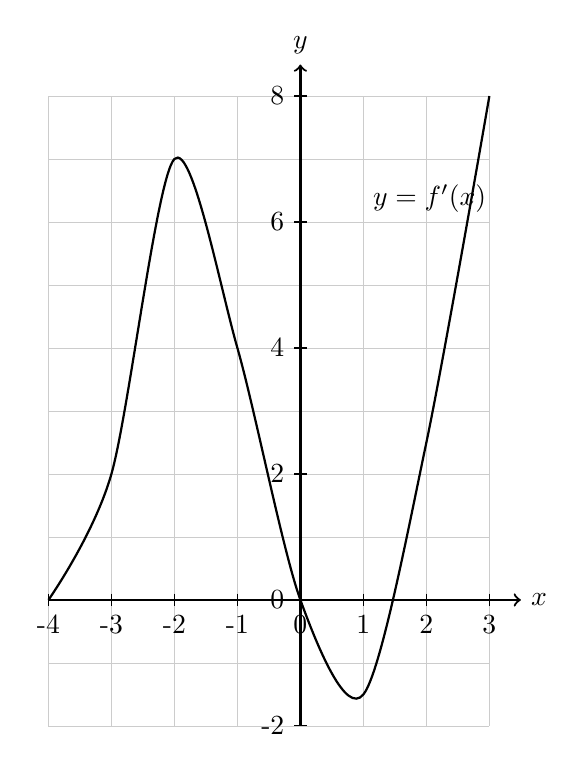
\begin{tikzpicture}[scale=0.8]
  \draw[step=1cm,gray!40,very thin] (-4,-2) grid (3,8);
  \draw[thick,->] (-4,0) -- (3.5,0) node[right] {$x$};
  \draw[thick,->] (0,-2) -- (0,8.5) node[above] {$y$};
  \node[above right] at (1,6) {$y=f'(x)$};
  \draw[thick,smooth]
    plot coordinates {(-4,0)(-3,2)(-2,7)(-1,4)
                      (0,0)(1,-1.5)(2,2.5)(3,8)};
  \foreach \x in {-4,-3,...,3}
    \draw (\x,0.1)--(\x,-0.1) node[below]{\x};
  \foreach \y in {-2,0,...,8}
    \draw (0.1,\y)--(-0.1,\y) node[left]{\y};
\end{tikzpicture}
\caption{Gráfica de la derivada $f'$: los ceros de $f'$ señalan los posibles
  extremos de $f$, el signo de $f'$ su monotonía, y el crecimiento o
  decrecimiento de $f'$ la concavidad de $f$.}
\label{fig:grafica_fprima}
\end{figure}
\end{prob}


% Desafiante
\begin{prob}[Geometría Analítica]
El piloto de un automóvil de carreras recorre una pista elíptica modelada
por la ecuación
\[
    \frac{x^2}{400} + \frac{y^2}{100} = 1.
\]
Al perder el control en el punto $(16,\,6)$, el vehículo continúa en línea
recta sobre la recta tangente a la elipse en ese punto.
\begin{enumerate}
    \item Verifique que el punto $(16,\,6)$ pertenece a la elipse.
    \item Determine la ecuación de la recta tangente a la elipse en dicho
          punto.
    \item Si el automóvil impacta contra un árbol ubicado en la coordenada
          $(14,\, k)$, determine el valor exacto de la constante $k$.
\end{enumerate}
\end{prob}

%%----------------------------------------------------------
\subsection{Optimización}
%%----------------------------------------------------------

% Básico
\begin{prob}
Encuentre las dimensiones del rectángulo de área máxima que puede
inscribirse en un círculo de radio $r$.
\end{prob}

\begin{prob}
Una lata cilíndrica con tapa debe contener $500$ cm$^3$. Encuentre
las dimensiones que minimizan el área total de material.
\end{prob}

\begin{prob}
Un terreno rectangular debe cercarse con $200$ m de malla. Un lado
del rectángulo es un muro existente el cual no necesita cerca. ¿Qué
dimensiones maximizan el área del terreno?
\end{prob}

\begin{prob}
Un rectángulo está inscrito bajo la parábola $y=8-x^2$ con su base
sobre el eje $x$. Encuentre las dimensiones del rectángulo de área
máxima.
\end{prob}

%\begin{prob}
%Sea $\ell > 0$ una constante dada. Se quiere diseñar un canal de sección transversal trapezoidal isósceles en el que el fondo y los dos taludes se recubren con material impermeable, quedando la superficie superior abierta al terreno. La longitud total revestida por metro lineal de canal es fija:
%\[
%  b + 2s = \ell, \qquad b > 0,\quad s > 0,
%\]
%donde $b$ es el ancho del fondo y $s$ la longitud de cada talud inclinado. El ángulo de inclinación de los taludes respecto a la horizontal es $\theta\in\bigl(0,\tfrac{\pi}{2}\bigr)$.
%
%La profundidad del canal es $h = s\sen\theta$, y el área de la sección
%transversal mojada es \[
%  A \;=\; (b + s\cos\theta)\,s\sen\theta.
%\]
%Como el caudal es proporcional a $A$, maximizar el caudal equivale a maximizar $A$. Se pide resolver los siguientes ítem:
%\begin{enumerate}
%  \item Usando la restricción $b = \ell - 2s$, exprese $A$ únicamente en función
%        de $s$ y $\theta$.
%  \item Determine los valores óptimos $b^{*}$, $s^{*}$ y $\theta^{*}$ en términos
%        de $\ell$.
%  \item Interprete geométricamente la configuración óptima.
%\end{enumerate}
%
%\begin{figure}[H]
%\centering
%\begin{tikzpicture}[scale=1.25, >=stealth, line join=round,
%                    every node/.style={font=\small}]
%
%  %--- parámetros visuales ---------------------------------------------------
%  \def\b{3.0}          % ancho del fondo
%  \def\s{2.0}          % longitud del talud
%  \def\th{60}          % ángulo en grados
%  \def\h{1.7321}       % h = s*sin(60°)
%  \pgfmathsetmacro{\dx}{\s*cos(\th)}   % proyección horizontal = s*cos(θ)
%
%  %--- vértices del trapecio --------------------------------------------------
%  \coordinate (A) at (0, 0);
%  \coordinate (B) at (\b, 0);
%  \coordinate (C) at (\b+\dx, \h);
%  \coordinate (D) at (-\dx, \h);
%
%  %--- área mojada ------------------------------------------------------------
%  \fill[blue!10] (A) -- (B) -- (C) -- (D) -- cycle;
%
%  %--- terreno natural --------------------------------------------------------
%  \fill[pattern=north east lines, pattern color=brown!50]
%    (-\dx-0.6, -0.3) rectangle (\b+\dx+0.6, 0);
%  \draw[brown!70, thick]
%    (-\dx-0.6, 0) -- (\b+\dx+0.6, 0);
%  \node[brown!80!black, below] at (0.5*\b, -0.18) {\footnotesize Terreno natural};
%
%  %--- lados revestidos (perímetro mojado = ℓ) --------------------------------
%  \draw[blue!70!black, line width=1.8pt] (D) -- (A) -- (B) -- (C);
%
%  %--- superficie libre (abierta) ---------------------------------------------
%  \draw[blue!40, dashed, thick] (D) -- (C);
%
%  %--- etiquetas de los taludes -----------------------------------------------
%  \node[blue!70!black, left=2pt]  at ($(D)!0.5!(A)$) {$s$};
%  \node[blue!70!black, right=2pt] at ($(B)!0.5!(C)$) {$s$};
%
%  %--- etiqueta del fondo -----------------------------------------------------
%  \node[blue!70!black, below=4pt] at (0.5*\b, 0) {$b$};
%
%  %--- ancho superior ---------------------------------------------------------
%  \draw[<->, gray, thin] (D) ++(0, 0.35) -- ++(\b+2*\dx, 0)
%        node[midway, above, gray] {$b + 2s\cos\theta$};
%
%  %--- altura h ---------------------------------------------------------------
%  \draw[<->, red!70!black, thin]
%    (-\dx-0.35, 0) -- (-\dx-0.35, \h)
%    node[midway, left] {$h = s\sen\theta$};
%
%  %--- línea auxiliar horizontal (para el ángulo) -----------------------------
%  \draw[gray, dashed, thin] (A) -- ++(-0.5, 0);
%
%  %--- ángulo θ ---------------------------------------------------------------
%  \draw[->, thin] (A) ++(-0.4, 0) arc (180:{180-\th}:0.4);
%  \node at (-0.18, 0.28) {$\theta$};
%
%  %--- nota del perímetro revestido -------------------------------------------
%  \node[anchor=north west, align=left, font=\footnotesize, text=blue!60!black]
%    at (-\dx-0.6, -0.55)
%    {$\ell = b + 2s$ \ (perímetro revestido por metro lineal)};
%
%\end{tikzpicture}
%\end{figure}
%\end{prob}



%\begin{prob}
%El costo de construir la pared frontal de un edificio es el triple del
%costo de las demás paredes. El edificio debe tener volumen $V_0$ m$^3$
%y planta rectangular. Encuentre la relación entre largo y ancho de la
%base que minimiza el costo total.
%\end{prob}

% Intermedio
\begin{prob}
Se desea construir una pecera sin tapa, con base cuadrada y paredes
verticales, de capacidad $2000$ m$^3$. La base es de concreto y las
paredes de vidrio. El costo por m$^2$ del vidrio es el doble del del
concreto. ¿Cuál debe ser la altura de la pecera para que el costo
total sea mínimo?
\end{prob}

\begin{prob}
En una hoja rectangular se deben dejar márgenes laterales de $2$
pulgadas y márgenes superior e inferior de $1$ pulgada. El área
impresa es de $32$ pulg$^2$. Encuentre las dimensiones de la hoja
que minimicen el área total del papel.
\end{prob}

\begin{prob}
El equipo Alianza Petrolera juega en un estadio con capacidad de
$12\,000$ espectadores. Con entrada a \$$20\,000$ la asistencia
promedio es de $4\,000$. Un estudio estima que si el precio baja
\$$2\,000$, la asistencia sube $1\,000$ espectadores. ¿Qué precio de
entrada y cuántos espectadores maximizan los ingresos por boletería?
\end{prob}

\begin{prob}
Se proyecta construir un jardín en forma de sector circular de radio
$r$ y ángulo central $\theta$. El área del jardín ha de ser
$10\,000$ m$^2$. Encuentre los valores de $r$ y $\theta$ que
minimizan el perímetro del jardín.
\end{prob}

% Desafiante
\begin{prob}
Un hombre debe escapar desde el punto $A$, ubicado en la costa de una isla, hasta
el punto $B$ en una isla vecina, donde un helicóptero lo espera hasta máximo
$4$~horas. La distancia de $A$ a $B$ es de $13$~km y el punto $B$ se encuentra
a $5$~km de la costa de manera perpendicular. El hombre puede trotar a $5$~km/h
a lo largo de la costa y nadar a $3$~km/h. Planea trotar desde $A$ hasta un
punto~$C$ en la costa y luego nadar en línea recta desde $C$ hasta $B$.

\begin{enumerate}[(a)]
  \item ¿A qué distancia de $A$ debe ubicarse el punto~$C$ para minimizar el
        tiempo total de viaje?
  \item ¿Llegará al helicóptero antes de que deba partir?
\end{enumerate}

\begin{figure}[H]
\centering
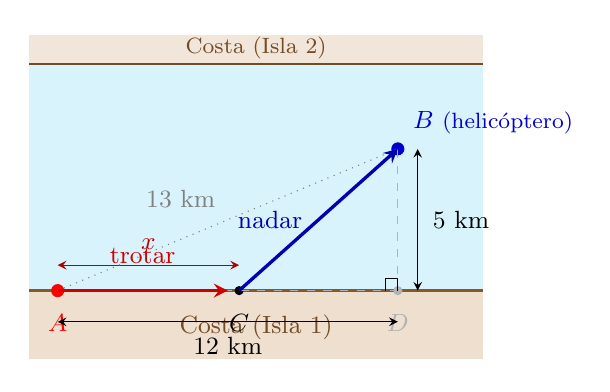
\begin{tikzpicture}[scale=0.72, >=stealth, line join=round,
                    every node/.style={font=\small}]

  %--- parámetros (escala visual) ---
  % Distancia A-D a lo largo de la costa: 12 km  → 6 unidades
  % Altura de B sobre la costa:            5 km  → 2.5 unidades
  % Escala: 1 unidad = 2 km
  \def\D{6}      % posición x de D (pie de perpendicular desde B)
  \def\H{2.5}    % altura de B

  %--- agua y costa ---
  \fill[cyan!15] (-0.5,0) rectangle (7.5,4.5);
  \fill[brown!25] (-0.5,-1.2) rectangle (7.5,0);
  \draw[very thick, brown!70!black] (-0.5,0) -- (7.5,0);
  \node[brown!60!black] at (3.5,-0.65) {Costa (Isla 1)};

  %--- punto A ---
  \filldraw[red] (0,0) circle (3pt) node[below=5pt] {$A$};

  %--- punto C (genérico, a distancia x de A) ---
  \filldraw[black] (3.2,0) circle (2pt) node[below=5pt] {$C$};

  %--- punto D (pie de la perpendicular desde B, a 12 km de A) ---
  \filldraw[gray!60] (\D,0) circle (2pt) node[below=5pt] {$D$};

  %--- punto B ---
  \filldraw[blue!80!black] (\D,\H) circle (3pt)
      node[above right=2pt] {$B$ \footnotesize(helicóptero)};

  %--- línea punteada de referencia: A hasta D (costa) ---
  \draw[dashed, gray!60] (0,0) -- (\D,0);

  %--- perpendicular de D a B ---
  \draw[dashed, gray!60] (\D,0) -- (\D,\H);
  \draw (\D,0) -- ++(0,0.22) -- ++(-0.22,0) -- ++(0,-0.22); % ángulo recto

  %--- cotas ---
  % cota vertical: 5 km (D a B)
  \draw[<->, thin] (\D+0.35,0) -- (\D+0.35,\H)
      node[midway, right=2pt] {$5$ km};

  % cota horizontal: 12 km (A a D)
  \draw[<->, thin] (0,-0.55) -- (\D,-0.55)
      node[midway, below=2pt] {$12$ km};

  % cota x (A a C)
  \draw[<->, thin, red!70!black] (0,0.45) -- (3.2,0.45)
      node[midway, above=2pt] {$x$};

  %--- hipotenusa de referencia A-B: 13 km ---
  \draw[dotted, gray] (0,0) -- (\D,\H)
      node[midway, above left=1pt, gray] {$13$ km};

  %--- trayectorias ---
  % Trotar: A -> C
  \draw[->, very thick, red!80!black] (0,0) -- (3.0,0)
      node[midway, above=6pt] {trotar};

  % Nadar: C -> B
  \draw[->, very thick, blue!70!black] (3.2,0) -- (\D,\H)
      node[midway, left=2pt] {nadar};

  %--- isla 2 (fondo) ---
  \fill[brown!20] (-0.5,4.0) rectangle (7.5,4.5);
  \draw[brown!60!black, thick] (-0.5,4.0) -- (7.5,4.0);
  \node[brown!60!black] at (3.5,4.28) {\footnotesize Costa (Isla 2)};

\end{tikzpicture}
\caption{Trayecto mixto: se trota de $A$ a $C$ (distancia $x$ a lo largo de
  la costa, $12$ km de $A$ a $D$) y se nada de $C$ al helicóptero $B$, situado
  $5$ km mar adentro. Se minimiza el tiempo total.}
\label{fig:trote_nado}
\end{figure}
\end{prob}

\begin{prob}
Ana asiste a una sala de cine cuya pantalla se modela como un segmento vertical de $2$ m de altura, ubicado sobre el eje $y$ entre los puntos $A(0,1)$ y $B(0,3)$ (todas las distancias están dadas en metros). Las butacas están distribuidas sobre la recta $y=x$ con $x>0$. Ana desea ocupar un lugar sobre dicha recta que maximice su ángulo de visión $\theta$ de la pantalla.

\begin{enumerate}
  \item Exprese $\theta$ en función de la coordenada $x$ de la posición de Ana.
  \item Determine el punto exacto $(x,x)$ donde debe sentarse para maximizar $\theta$.
  \item Calcule la distancia horizontal desde la pantalla hasta dicho punto óptimo.
\end{enumerate}

\textit{Sugerencia:} Use la identidad trigonométrica
\[
\tan(\alpha+\theta)=\frac{\tan\alpha+\tan\theta}{1-\tan\alpha\tan\theta}
\]
aplicada a los ángulos que forman las líneas de visión con la horizontal.

\begin{figure}[H]
\centering
\begin{tikzpicture}[scale=1.1, >=stealth, line join=round, every node/.style={font=\small}]
  % Ejes coordenados
  \draw[->] (-0.5,0) -- (3.5,0) node[below] {$x$};
  \draw[->] (0,-0.5) -- (0,3.5) node[left] {$y$};
  
  % Marcas y etiquetas en los ejes
  \foreach \i in {0.5,1,...,3} {
    \draw (\i,0.05) -- (\i,-0.05) node[below] {\i};
    \draw (0.05,\i) -- (-0.05,\i) node[left] {\i};
  }
  
  % Recta y = x
  \draw[thick, teal!70!black] (-0.3,-0.3) -- (3.5,3.5) node[above left] {$y=x$};
  
  % Pantalla (segmento en el eje y)
  \draw[very thick] (0,1) -- (0,3);
  \fill[blue!70!black] (0,1) circle (2.2pt) node[above right] {A};
  \fill[blue!70!black] (0,3) circle (2.2pt) node[above right] {B};
  \node at (0.45, 2.15) {Pantalla};
  
  % Punto de Ana (C) sobre y=x
  \coordinate (C) at (2,2);
  \fill[blue!70!black] (C) circle (2.2pt) node[above right] {C};
  \node[below right] at (C) {Ana};
  
  % Líneas de visión (trazado discontinuo)
  \draw[dashed, thick, gray!60!black] (C) -- (0,1);
  \draw[dashed, thick, gray!60!black] (C) -- (0,3);
  

  
  % Ángulo θ en C
  \path (0,1) coordinate (A) (0,3) coordinate (B);
  \pic [draw, thick, angle radius=0.6cm, angle eccentricity=1.3, "$\theta$"] {angle = B--C--A};

\end{tikzpicture}
\caption{Ángulo de visión $\theta$ de la pantalla $AB$ (segmento vertical
  entre $A(0,1)$ y $B(0,3)$) desde un asiento $C=(x,x)$ sobre la recta $y=x$.}
\label{fig:cine_angulo}
\end{figure}
\end{prob}

\begin{prob}[Optimización de la longitud del cable]
Dos astas de bandera se encuentran instaladas verticalmente sobre un terreno plano. La distancia entre las bases de las astas es de $3$ metros. Se desea sujetar ambas astas con un cable que parte de la parte superior de cada asta y se ancla en un único punto sobre el suelo situado entre ambas.

Se conoce que la altura de la primera asta es de $2$ metros y la altura de la segunda es de $1$ metro. Determine la distancia $x$ desde la base de la asta más alta hasta el punto de anclaje en el suelo, de modo que la longitud total del cable ($d_1 + d_2$) sea mínima.

\begin{figure}[H]
\centering
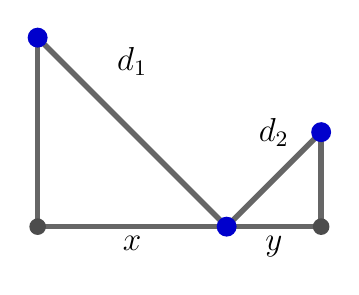
\begin{tikzpicture}[scale=1.2, >=stealth, line join=round]
  % Definición de puntos geométricos
  \coordinate (Top1) at (0,2);
  \coordinate (Base1) at (0,0);
  \coordinate (Top2) at (3,1);
  \coordinate (Base2) at (3,0);
  % Punto de anclaje en el suelo (x=2, y=1 es la solución óptima matemática)
  \coordinate (Anchor) at (2,0);

  % Estilos para las líneas gruesas (postes y cables)
  \tikzset{thicklines/.style={line width=2pt, color=gray!80!black}}
  
  % Dibujar postes y cables
  \draw[thicklines] (Base1) -- (Top1); % Asta 1
  \draw[thicklines] (Base2) -- (Top2); % Asta 2
  \draw[thicklines] (Base1) -- (Base2); % Suelo
  \draw[thicklines] (Top1) -- (Anchor); % Cable d1
  \draw[thicklines] (Top2) -- (Anchor); % Cable d2

  % Puntos (nodos circulares)
  % Puntos azules (extremos activos y punto de unión)
  \fill[blue!80!black] (Top1) circle (3pt);
  \fill[blue!80!black] (Top2) circle (3pt);
  \fill[blue!80!black] (Anchor) circle (3pt);
  
  % Puntos grises (bases fijas)
  \fill[gray!60!black] (Base1) circle (2.5pt);
  \fill[gray!60!black] (Base2) circle (2.5pt);

  % Etiquetas de distancias
  \node[above, font=\large, color=black!80!black] at (1, 1.5) {$d_1$};
  \node[above, font=\large, color=black!80!black] at (2.5, 0.75) {$d_2$};
  \node[below, font=\large, color=black!80!black] at (1, 0) {$x$};
  \node[below, font=\large, color=black!80!black] at (2.5, 0) {$y$};

\end{tikzpicture}
\caption{Dos astas verticales (alturas $2$ m y $1$ m, bases separadas $3$ m)
  unidas por un cable anclado en el suelo a distancia $x$ de la base más alta;
  se minimiza la longitud total $d_1+d_2$.}
\label{fig:astas_cable}
\end{figure}
\end{prob}


%%----------------------------------------------------------
\subsection{Teorema del Valor Medio}
%%----------------------------------------------------------

% Básico
\begin{prob}
Verifique el TVM para $f(x)=\sqrt{x}$ en $[1,4]$ y encuentre el valor
de $c$ garantizado por el teorema.
\end{prob}

% Intermedio
\begin{prob}
Use el TVM para demostrar que $|\sen a - \sen b| \leq |a-b|$ para
todo $a,b\in\R$.
\end{prob}

\begin{prob}
Demuestre que la ecuación $x^5+10x+3=0$ tiene exactamente una raíz
real. \textit{Sugerencia:} use el TVI para existencia y el TVM para
unicidad.
\end{prob}

\begin{prob}
Un automóvil sale de un semáforo en rojo y, $60$ s después, pasa
frente a un radar que registra $80$ km/h. Demuestre que en algún
momento entre los $0$ y $60$ s su aceleración fue positiva.
\end{prob}

\begin{prob}
Sea $f(x)=\alpha x^2+\beta x+\gamma$ con $\alpha\neq 0$. Demuestre que
el número $c$ garantizado por el Teorema del Valor Medio en cualquier
intervalo $[a,b]$ es siempre el punto medio $\dfrac{a+b}{2}$.
\end{prob}

% Desafiante
\begin{prob}
La función $f(x)=x^2-1$ no satisface las hipótesis del TVM
    en $[-1,8]$; sin embargo, ¿es posible encontrar $c\in(-1,8)$ tal
    que $f'(c)=10$?
    \end{prob}
    \begin{prob}
Usando trigonometría, ¿por qué para $x\neq\pi/2$ es posible
    encontrar $c\in(-1,8)$ tal que $\cos c=1$? ¿Contradice esto el TVM?
\end{prob}


%%----------------------------------------------------------
\subsection{Regla de L'Hôpital}
%%----------------------------------------------------------

% Básico
\begin{prob}
Calcule cada límite:
\begin{multicols}{2}
\begin{enumerate}
    \item $\displaystyle\lim_{x\to 0}\frac{x-\sen x}{x^3}$
    \item $\displaystyle\lim_{x\to\infty}\frac{\ln x}{x^p}$, $p>0$
    \item $\displaystyle\lim_{x\to 0^+}x^p\ln x$, $p>0$
    \item $\displaystyle\lim_{x\to\infty}x^{1/x}$
    \item $\displaystyle\lim_{x\to 0}\frac{e^x-e^{-x}-2x}{x-\sen x}$
    \item $\displaystyle\lim_{x\to 0}(\csc x - \cot x)$
    \item $\displaystyle\lim_{x\to 0}\left(\frac{1}{x^2}-\cot^2 x\right)$
    \item $\displaystyle\lim_{x\to 1}\frac{x^x-x}{1-x+\ln x}$
    \item $\displaystyle\lim_{x\to\infty}\left(\sqrt{x^2+x}-x\right)$
    \item $\displaystyle\lim_{x\to 0^+}(\tan x)^{\sen x}$
\end{enumerate}
\end{multicols}
\end{prob}

% Intermedio
\begin{prob}
Observe que en el límite
\[
\lim_{x\to 0}\frac{\sqrt{12-x^2}-\sqrt{12}}{x^2}
\]
el numerador y el denominador se anulan en $x=0$. ¿Cuál de las
condiciones de la regla de L'Hôpital no se satisface? Determine el
valor del límite y justifique.
\end{prob}

\begin{prob}
Deduzca si cada afirmación es verdadera o falsa y justifique:
\begin{enumerate}[a)]
    \item Si $\lim_{x\to a}\dfrac{f(x)}{g(x)}$ es de la forma
    $\dfrac{0}{0}$, entonces $\lim_{x\to a}\dfrac{f(x)}{g(x)}
    = \lim_{x\to a}\dfrac{f'(x)}{g'(x)}$.
    \item Si $\lim_{x\to a}f(x)=2$ y $\lim_{x\to a}g(x)=0$, puede
    aplicarse L'Hôpital a $\lim_{x\to a}\dfrac{f(x)}{g(x)}$.
    \item Si L'Hôpital se aplica y el nuevo límite no existe, entonces
    el límite original tampoco existe.
\end{enumerate}
\end{prob}

% Desafiante
\begin{prob}
Demuestre que $\displaystyle\lim_{x\to\infty}(1+x)^{1/x} = 1$ usando
diferenciación logarítmica para analizar el comportamiento de $\ln y$.
Compare con el límite $\lim_{n\to\infty}\!\left(1+\dfrac{1}{n}\right)^n = e$.
\end{prob}


%%----------------------------------------------------------
\subsection{Métodos numéricos para la localización de raíces}
%%----------------------------------------------------------

% Básico
\begin{prob}
Use la bisección para aproximar la raíz de $f(x)=x^3+x-1$ en $[0,1]$
con un error menor que $0.01$. Construya una tabla de iteraciones.
\end{prob}

% Intermedio
\begin{prob}
Aplique el método de Newton-Raphson a $f(x)=\cos x - x$ con $x_0=1$
hasta obtener $5$ cifras decimales correctas. Verifique la convergencia
cuadrática comparando los errores en cada iteración.
\end{prob}

\begin{prob}
La ecuación $x = \cos x$ puede reescribirse como punto fijo de dos
maneras distintas: $g_1(x)=\cos x$ y $g_2(x)=\arccos x$. Para cada
una, analice si la condición $|g'|<1$ se cumple cerca de la raíz
$c\approx 0.739$ y prediga cuál convergerá.
\end{prob}

% Desafiante
\begin{prob}
Demuestre que la iteración de Newton-Raphson aplicada a $f(x)=x^2-a$
(con $a>0$) produce la sucesión
\[
x_{n+1}=\frac{1}{2}\!\left(x_n+\frac{a}{x_n}\right),
\]
conocida como \textbf{algoritmo babilónico} de la raíz cuadrada.
Verifique que converge cuadráticamente.
\end{prob}










